\documentclass[11pt,twoside=semi,openright,numbers=noenddot,titlepage=false]{scrbook}
\newcommand{\napkinversion}{v1.0.\hbox{\the\year\twodigits\month\twodigits\day}}

%%fakesection Load packages

\usepackage{lmodern}
\usepackage[pdfusetitle]{hyperref}
\ExplSyntaxOn
\sys_if_engine_luatex:T {
	\usepackage{luatex85}
}
\sys_if_engine_pdftex:T {
	\usepackage[T1]{fontenc}
}
\ExplSyntaxOff

% These are evan.sty
\usepackage{amsmath,amssymb,amsthm}
\usepackage{mathrsfs}
\usepackage[usenames,svgnames,dvipsnames]{xcolor}
\usepackage{textcomp}
\usepackage{enumerate}
\usepackage[textsize=scriptsize,shadow]{todonotes}
\usepackage{mathtools}
\usepackage{microtype}
\usepackage[normalem]{ulem}
\usepackage{stmaryrd}
\usepackage{wasysym}
\usepackage{multirow}
\usepackage{prerex}
\usepackage[nameinlink]{cleveref}
\usepackage{derivative}

%%fakesection evan.sty macros
%Small commands
%% Napkin commands
\newcommand{\prototype}[1]{
	\emph{{\color{red} Prototypical example for this section:} #1} \par\medskip
}
\newenvironment{moral}{%
	\begin{mdframed}[linecolor=green!70!black]%
	\bfseries\color{green!50!black}}%
	{\end{mdframed}}

%%fakesection Links (hyperref loaded earlier implicitly)
\hypersetup{
	linkcolor={red!50!black},
	citecolor={green!50!black},
	urlcolor={blue!80!black},
	pdfkeywords={napkin,math},
	pdfsubject={web.evanchen.cc},
	colorlinks,
}

%%fakesection Commutative diagrams
\usepackage{tikz-cd}
\usetikzlibrary{arrows,arrows.meta}
% make a larger hook
% https://tex.stackexchange.com/questions/514451/how-to-define-a-new-hooked-arrow
\makeatletter
\pgfdeclarearrow{
	name=xGlyph,
	cache=false,
	bending mode=none,
	parameters={\tikzcd@glyph@len,\tikzcd@glyph@shorten},
	setup code={%
		\pgfarrowssettipend{\tikzcd@glyph@len\advance\pgf@x by\tikzcd@glyph@shorten}},
	defaults={
		glyph axis=axis_height,
		glyph length=+1.55ex,
		glyph shorten=+-0.1ex},
	drawing code={%
		\pgfpathrectangle{\pgfpoint{+0pt}{+-1.5ex}}{\pgfpoint{+\tikzcd@glyph@len}{+3ex}}%
		\pgfusepathqclip%
		\pgftransformxshift{+\tikzcd@glyph@len}%
		\pgftransformyshift{+-\tikzcd@glyph@axis}%
		\pgftext[right,base]{\tikzcd@glyph}}}
\makeatother
\tikzcdset{
	arrow style=tikz,
	diagrams={>={Latex}},
	tikzcd left hook/.tip={xGlyph[glyph math command=supset, swap, glyph axis = 5.7pt]},
	tikzcd right hook/.tip={xGlyph[glyph math command=supset, glyph axis = 5.7pt]},
	surjective head arrow /.tip = {tikzcd to[sep=-1.5pt]tikzcd to},
	surjective head/.style={
		-surjective head arrow
	}
}

%%fakesection Page layout
\usepackage[headsepline]{scrlayer-scrpage}
\renewcommand{\headfont}{}
\addtolength{\textheight}{3.14cm}
\setlength{\footskip}{0.5in}
\setlength{\headsep}{10pt}

\def\shortdate{\leavevmode\hbox{\the\year-\twodigits\month-\twodigits\day}}
\def\twodigits#1{\ifnum#1<10 0\fi\the#1}
\automark[chapter]{chapter}

\rohead{\footnotesize\thepage}
\rehead{\footnotesize \textbf{\sffamily Napkin}, by \emph{Evan Chen} (\napkinversion)}
\lehead{\footnotesize\thepage}
\lohead{\footnotesize \leftmark}
\chead{}
\rofoot{}
\refoot{}
\lefoot{}
\lofoot{}
%\cfoot{\pagemark}

%%fakesection Fancy section and chapter heads
\renewcommand*{\sectionformat}{\color{purple}\S\thesection\autodot\enskip}
\renewcommand*{\subsectionformat}{\color{purple}\S\thesubsection\autodot\enskip}
\newcommand{\problemhead}{A few harder problems to think about}
\renewcommand{\thesubsection}{\thesection.\roman{subsection}}

\addtokomafont{chapterprefix}{\raggedleft}
\RedeclareSectionCommand[beforeskip=0.5em]{chapter}
\renewcommand*{\chapterformat}{%
\mbox{\scalebox{1.5}{\chapappifchapterprefix{\nobreakspace}}%
\scalebox{2.718}{\color{purple}\thechapter\autodot}\enskip}}

\addtokomafont{partprefix}{\rmfamily}
\renewcommand*{\partformat}{\color{purple}\scalebox{2.5}{\thepart}}

%%fakesection Theorems
\usepackage{thmtools}
\usepackage[framemethod=TikZ]{mdframed}

\theoremstyle{definition}
\mdfdefinestyle{mdbluebox}{%
	roundcorner = 10pt,
	linewidth=1pt,
	skipabove=12pt,
	innerbottommargin=9pt,
	skipbelow=2pt,
	nobreak=true,
	linecolor=blue,
	backgroundcolor=TealBlue!5,
}
\declaretheoremstyle[
	headfont=\sffamily\bfseries\color{MidnightBlue},
	mdframed={style=mdbluebox},
	headpunct={\\[3pt]},
	postheadspace={0pt}
]{thmbluebox}

\mdfdefinestyle{mdredbox}{%
	linewidth=0.5pt,
	skipabove=12pt,
	frametitleaboveskip=5pt,
	frametitlebelowskip=0pt,
	skipbelow=2pt,
	frametitlefont=\bfseries,
	innertopmargin=4pt,
	innerbottommargin=8pt,
	linecolor=RawSienna,
	backgroundcolor=Salmon!5,
}
\declaretheoremstyle[
	headfont=\bfseries\color{RawSienna},
	mdframed={style=mdredbox},
	headpunct={\\[3pt]},
	postheadspace={0pt},
]{thmredbox}

\declaretheorem[%
style=thmbluebox,name=Theorem,numberwithin=section]{theorem}
\declaretheorem[style=thmbluebox,name=Lemma,sibling=theorem]{lemma}
\declaretheorem[style=thmbluebox,name=Proposition,sibling=theorem]{proposition}
\declaretheorem[style=thmbluebox,name=Corollary,sibling=theorem]{corollary}
\declaretheorem[style=thmredbox,name=Example,sibling=theorem]{example}

\mdfdefinestyle{mdgreenbox}{%
	skipabove=8pt,
	linewidth=2pt,
	rightline=false,
	leftline=true,
	topline=false,
	bottomline=false,
	linecolor=ForestGreen,
	backgroundcolor=ForestGreen!5,
}
\declaretheoremstyle[
	headfont=\bfseries\sffamily\color{ForestGreen!70!black},
	bodyfont=\normalfont,
	spaceabove=2pt,
	spacebelow=1pt,
	mdframed={style=mdgreenbox},
	headpunct={ --- },
]{thmgreenbox}
\declaretheoremstyle[
	headfont=\bfseries\sffamily\color{ForestGreen!70!black},
	bodyfont=\normalfont,
	spaceabove=2pt,
	spacebelow=1pt,
	mdframed={style=mdgreenbox},
	headpunct={},
]{thmgreenbox*}

\mdfdefinestyle{mdblackbox}{%
	skipabove=8pt,
	linewidth=3pt,
	rightline=false,
	leftline=true,
	topline=false,
	bottomline=false,
	linecolor=black,
	backgroundcolor=RedViolet!5!gray!5,
}
\declaretheoremstyle[
	headfont=\bfseries,
	bodyfont=\normalfont\small,
	spaceabove=0pt,
	spacebelow=0pt,
	mdframed={style=mdblackbox}
]{thmblackbox}

\declaretheorem[name=Question,sibling=theorem,style=thmblackbox]{ques}
\declaretheorem[name=Exercise,sibling=theorem,style=thmblackbox]{exercise}
\declaretheorem[name=Remark,sibling=theorem,style=thmgreenbox]{remark}
\declaretheorem[name=Remark,sibling=theorem,style=thmgreenbox*]{remark*}
\declaretheorem[name=Step,style=thmgreenbox]{step} % only used in Lebesgue int

\theoremstyle{definition}
\newtheorem{claim}[theorem]{Claim}
\newtheorem{definition}[theorem]{Definition}
\newtheorem{fact}[theorem]{Fact}
\newtheorem{abuse}[theorem]{Abuse of Notation}

\newtheorem{problem}{Problem}[chapter]
\renewcommand{\theproblem}{\thechapter\Alph{problem}}
\newtheorem{sproblem}[problem]{Problem}
\newtheorem{dproblem}[problem]{Problem}
\renewcommand{\thesproblem}{\theproblem$^{\star}$}
\renewcommand{\thedproblem}{\theproblem$^{\dagger}$}
\newcommand{\listhack}{$\empty$\vspace{-2em}}

%%fakesection Answers
\usepackage{answers}
\Newassociation{hint}{answeritem}{tex/backmatter/all-hints}
\Newassociation{sol}{answeritem}{tex/backmatter/all-solns}
\renewcommand{\solutionextension}{out}
\renewenvironment{answeritem}[1]{\item[\bfseries #1.]}{}

%%fakesection Table of contents
% First add ToC to ToC
\makeatletter
\usepackage{etoolbox}
\pretocmd{\tableofcontents}{%
	\if@openright\cleardoublepage\else\clearpage\fi
	\pdfbookmark[0]{\contentsname}{toc}%
}{}{}%
\makeatother
\setcounter{tocdepth}{1}
\RedeclareSectionCommand[tocnumwidth=4.2em]{part}
\RedeclareSectionCommand[tocpagenumberwidth=2.2em,tocnumwidth=4.2em]{chapter}
\RedeclareSectionCommand[tocpagenumberwidth=2.2em,tocnumwidth=2.8em]{section}
% adjust tocpagenumberwidth manually for large page number: https://tex.stackexchange.com/a/502168

%%fakesection Asymptote definitions
\usepackage{patch-asy}
\numberwithin{asy}{chapter}
\renewcommand{\theasy}{\thechapter\Alph{asy}}
\begin{asydef}
	import extras;
	size(6cm);
	usepackage("amsmath");
	usepackage("amssymb");
	defaultpen(fontsize(11pt));
	settings.tex = "latex";
	settings.outformat = "pdf";
\end{asydef}
\def\asydir{asy}

%%fakesection Bibliography
\usepackage[backend=biber,backref=true,style=alphabetic]{biblatex}
\DeclareLabelalphaTemplate{
	\labelelement{
		\field[final]{shorthand}
		\field{label}
		\field[strwidth=2,strside=left]{labelname}
	}
	\labelelement{
		\field[strwidth=2,strside=right]{year}
	}
}
\DeclareFieldFormat{labelalpha}{\textbf{\scriptsize #1}}
\addbibresource{references.bib}
\addbibresource{images.bib}
%% stylistic biblatex choices
\DefineBibliographyStrings{english}{%
	backrefpage  = {cited p.}, % for single page number
	backrefpages = {cited pp.} % for multiple page numbers
}
\DeclareFieldFormat{journaltitle}{\mkbibemph{#1},} % italic journal title with comma
\DeclareFieldFormat[inbook,thesis]{title}{\mkbibemph{#1}\addperiod} % italic title with period
\DeclareFieldFormat[article]{title}{#1} % title of journal article is printed as normal text
\DeclareFieldFormat[article]{volume}{\textbf{#1}\addcolon\space}
\renewcommand{\mkbibnamegiven}[1]{\textsc{#1}}
\renewcommand{\mkbibnamefamily}[1]{\textsc{#1}}
\renewcommand{\mkbibnameprefix}[1]{\textsc{#1}}
\renewcommand{\mkbibnamesuffix}[1]{\textsc{#1}}
\renewcommand{\finentrypunct}{}

%%fakesection Mini ToC
\usepackage[tight]{minitoc}
\mtcsetfont{parttoc}{chapter}{\sffamily\bfseries}
\mtcsetfont{parttoc}{section}{\footnotesize\rmfamily\upshape\mdseries}
\mtcsetfont{parttoc}{subsection}{\footnotesize\rmfamily\upshape\mdseries}
%\mtcsetdepth{parttoc}{1}
\setcounter{parttocdepth}{1}
\renewcommand*{\partheadstartvskip}{\vspace*{20em}}
\renewcommand*{\partheadendvskip}{}
%\noptcrule
\renewcommand\beforeparttoc{\noindent{\bfseries \Large Part \thepart: Contents}}
%\hspace{\fill}\rule{0.95\linewidth}{2pt}\hspace{\fill}
\doparttoc[n]

%%fakesection Misc haxx
\pdfstringdefDisableCommands{\def\Spec{\text{Spec }}\def\sigma{σ}}

\newcommand{\cbrt}[1]{\sqrt[3]{#1}}
\newcommand{\floor}[1]{\left\lfloor #1 \right\rfloor}
\newcommand{\ceiling}[1]{\left\lceil #1 \right\rceil}
\newcommand{\mailto}[1]{\href{mailto:#1}{\texttt{#1}}}
\newcommand{\ol}{\overline}
\newcommand{\ul}{\underline}
\newcommand{\wt}{\widetilde}
\newcommand{\wh}{\widehat}
\newcommand{\eps}{\varepsilon}
%\renewcommand{\iff}{\Leftrightarrow}
%\renewcommand{\implies}{\Rightarrow}
\newcommand{\vocab}[1]{\textbf{\color{blue} #1}}
\newcommand{\catname}{\mathsf}
\newcommand{\hrulebar}{
  \par\hspace{\fill}\rule{0.95\linewidth}{.7pt}\hspace{\fill}
  \par\nointerlineskip \vspace{\baselineskip}
}
\newcommand{\half}{\frac{1}{2}}

%More commands and math operators
\DeclareMathOperator{\cis}{cis}
\DeclareMathOperator*{\lcm}{lcm}
\DeclareMathOperator*{\argmin}{arg min}
\DeclareMathOperator*{\argmax}{arg max}

%Convenient Environments
\newenvironment{soln}{\begin{proof}[Solution]}{\end{proof}}
\newenvironment{parlist}{\begin{inparaenum}[(i)]}{\end{inparaenum}}
\newenvironment{gobble}{\setbox\z@\vbox\bgroup}{\egroup}

%Inequalities
\newcommand{\cycsum}{\sum_{\mathrm{cyc}}}
\newcommand{\symsum}{\sum_{\mathrm{sym}}}
\newcommand{\cycprod}{\prod_{\mathrm{cyc}}}
\newcommand{\symprod}{\prod_{\mathrm{sym}}}

%From H113 "Introduction to Abstract Algebra" at UC Berkeley
\newcommand{\CC}{\mathbb C}
\newcommand{\FF}{\mathbb F}
\newcommand{\NN}{\mathbb N}
\newcommand{\QQ}{\mathbb Q}
\newcommand{\RR}{\mathbb R}
\newcommand{\ZZ}{\mathbb Z}
\newcommand{\charin}{\text{ char }}
\DeclareMathOperator{\sign}{sign}
\DeclareMathOperator{\Aut}{Aut}
\DeclareMathOperator{\Inn}{Inn}
\DeclareMathOperator{\Syl}{Syl}
\DeclareMathOperator{\Gal}{Gal}
\DeclareMathOperator{\GL}{GL} % General linear group
\DeclareMathOperator{\SL}{SL} % Special linear group

%From Kiran Kedlaya's "Geometry Unbound"
\newcommand{\abs}[1]{\left\lvert #1 \right\rvert}
\newcommand{\norm}[1]{\left\lVert #1 \right\rVert}
\newcommand{\dang}{\measuredangle} %% Directed angle
\newcommand{\ray}[1]{\overrightarrow{#1}}
\newcommand{\seg}[1]{\overline{#1}}
\newcommand{\arc}[1]{\wideparen{#1}}

%From M275 "Topology" at SJSU
\newcommand{\id}{\mathrm{id}}
\newcommand{\taking}[1]{\xrightarrow{#1}}
\newcommand{\inv}{^{-1}}

%From M170 "Introduction to Graph Theory" at SJSU
\DeclareMathOperator{\diam}{diam}
\DeclareMathOperator{\ord}{ord}
%\newcommand{\defeq}{\overset{\mathrm{def}}{=}}
\newcommand{\defeq}{\coloneq}

%From the USAMO .tex files
\newcommand{\st}{^{\text{st}}}
\newcommand{\nd}{^{\text{nd}}}
\renewcommand{\th}{^{\text{th}}}
\newcommand{\dg}{^\circ}
\newcommand{\ii}{\item}

% From Math 55 and Math 145 at Harvard
\newenvironment{subproof}[1][Proof]{%
\begin{proof}[#1] \renewcommand{\qedsymbol}{$\blacksquare$}}%
{\end{proof}}

\newcommand{\liff}{\leftrightarrow}
\newcommand{\lthen}{\rightarrow}
\newcommand{\opname}{\operatorname}
\newcommand{\surjto}{\twoheadrightarrow}
\newcommand{\injto}{\hookrightarrow}
\newcommand{\On}{\mathrm{On}} % ordinals
\DeclareMathOperator{\img}{im} % Image
\DeclareMathOperator{\Img}{Im} % Image
\DeclareMathOperator{\coker}{coker} % Cokernel
\DeclareMathOperator{\Coker}{Coker} % Cokernel
\DeclareMathOperator{\Ker}{Ker} % Kernel
\DeclareMathOperator{\rank}{rank}
\DeclareMathOperator{\Spec}{Spec} % spectrum
\DeclareMathOperator{\Tr}{Tr} % trace
\DeclareMathOperator{\pr}{pr} % projection
\DeclareMathOperator{\ext}{ext} % extension
\DeclareMathOperator{\pred}{pred} % predecessor
\DeclareMathOperator{\dom}{dom} % domain
\DeclareMathOperator{\ran}{ran} % range
\DeclareMathOperator{\Hom}{Hom} % homomorphism
\DeclareMathOperator{\End}{End} % endomorphism

% Things Lie
\newcommand{\kg}{\mathfrak g}
\newcommand{\kh}{\mathfrak h}
\newcommand{\kn}{\mathfrak n}
\newcommand{\ku}{\mathfrak u}
\newcommand{\kz}{\mathfrak z}
\DeclareMathOperator{\Ext}{Ext} % Ext functor
\DeclareMathOperator{\Tor}{Tor} % Tor functor

% More script letters etc.
\newcommand{\SA}{\mathscr A}
\newcommand{\SB}{\mathscr B}
\newcommand{\SC}{\mathscr C}
\newcommand{\SD}{\mathscr D}
\newcommand{\SF}{\mathscr F}
\newcommand{\SG}{\mathscr G}
\newcommand{\SH}{\mathscr H}
\newcommand{\OO}{\mathcal O}


%%fakesection Napkin Macros
\newcommand{\Zc}[1]{\ZZ/#1\ZZ}
\newcommand{\Zcc}[1]{\ZZ/(#1)\ZZ}
\newcommand{\Zm}[1]{(\ZZ/#1\ZZ)^\times}
\newcommand{\EE}{\mathbb E}
\newcommand{\TT}{\mathbb T}
\newcommand{\im}{^{\text{img}}} % or ``?
\newcommand{\pre}{^{\text{pre}}}
\newcommand{\normalin}{\trianglelefteq}
\newcommand{\triv}{\mathrm{triv}}
\newcommand{\largeotimes}[1]{\mathop{\otimes}\limits_{#1}}
\newcommand{\Mat}{\mathrm{Mat}}
\newcommand{\PGL}[1]{\mathbf{PGL}_{#1}(\CC)}

\DeclareMathOperator{\Stab}{Stab}
\DeclareMathOperator{\FixPt}{FixPt}
\DeclareMathOperator{\refl}{refl}
\DeclareMathOperator{\Fun}{Fun}
\DeclareMathOperator{\Irrep}{Irrep}
\DeclareMathOperator{\Res}{Res}
\DeclareMathOperator{\Reg}{Reg}
\DeclareMathOperator{\Classes}{Classes}
\DeclareMathOperator{\Frac}{Frac}
\newcommand{\FunCl}{\Fun_{\mathrm{class}}}
\newcommand{\Homrep}{\Hom_{\mathrm{rep}}}
\newcommand{\ab}{^\text{ab}} % abelianization
\DeclareMathOperator{\ev}{ev}
\DeclareMathOperator{\Wind}{\mathbf I}
\newcommand{\Ctriv}{\CC_{\mathrm{triv}}}
\newcommand{\Csign}{\CC_{\mathrm{sign}}}
\DeclareMathOperator{\Alt}{Alt}

% Riemann surface
\DeclareMathOperator{\Div}{div} % divisor
\DeclareMathOperator{\mult}{mult}

% Alg geom macros
\newcommand{\VV}{\mathcal V}
\newcommand{\Vp}{\mathcal V_{\text{pr}}}
\newcommand{\Aff}{\mathbb A}
\newcommand{\II}{\mathcal I_{\text{rad}}}
\newcommand{\RP}{\mathbb{RP}}
\newcommand{\CP}{\mathbb{CP}}
\newcommand{\Cl}{\mathrm{Cl}}
\newcommand{\restrict}[1]{\bgroup\restriction_{#1}\egroup}
\DeclareMathOperator{\Opens}{OpenSets}
\DeclareMathOperator{\Proj}{Proj}
\DeclareMathOperator{\res}{res}
\newcommand{\km}{\mathfrak m}
\newcommand{\sh}{^\mathrm{sh}}

\renewcommand{\Re}{\opname{Re}}
\renewcommand{\Im}{\opname{Im}}

%% Category Theory macros
\renewcommand{\AA}{\mathcal A}
\newcommand{\BB}{\mathcal B}
\newcommand{\obj}{\operatorname{obj}}
\newcommand{\op}{^{\mathrm{op}}}


\usepackage{tkz-graph}
\pgfarrowsdeclare{biggertip}{biggertip}{%
  \setlength{\arrowsize}{1pt}
  \addtolength{\arrowsize}{.1\pgflinewidth}
  \pgfarrowsrightextend{0}
  \pgfarrowsleftextend{-5\arrowsize}
}{%
  \setlength{\arrowsize}{1pt}
  \addtolength{\arrowsize}{.1\pgflinewidth}
  \pgfpathmoveto{\pgfpoint{-5\arrowsize}{4\arrowsize}}
  \pgfpathlineto{\pgfpointorigin}
  \pgfpathlineto{\pgfpoint{-5\arrowsize}{-4\arrowsize}}
  \pgfusepathqstroke
}
\tikzset{
	EdgeStyle/.style = {>=biggertip}
}

\usepackage[all,cmtip,2cell]{xy}
\UseTwocells
\newcommand\nattfm[5]{\xymatrix@C+2pc{#1 \rtwocell<4>^{#2}_{#4}{\; #3} & #5}}

%% Alg Top macros
\DeclareMathOperator{\Cells}{Cells}
\newcommand{\HdR}{H_{\mathrm{dR}}}

%% Alg NT macros
\newcommand{\ka}{\mathfrak a}
\newcommand{\kb}{\mathfrak b}
\newcommand{\kp}{\mathfrak p}
\newcommand{\kq}{\mathfrak q}

\newcommand{\Frob}{\mathrm{Frob}}
\DeclareMathOperator{\Norm}{N}
\DeclareMathOperator{\Ram}{Ram}
\newcommand{\TrK}{\Tr_{K/\QQ}}
\newcommand{\NK}{\Norm_{K/\QQ}}
\newcommand{\kf}{\mathfrak f}
\newcommand{\kP}{\mathfrak P}
\newcommand{\kQ}{\mathfrak Q}

%% Diff geo macros
\newcommand{\ee}{\mathbf e}
\newcommand{\fpartial}[2]{\frac{\partial #1}{\partial #2}}

%% ST macros
\newcommand{\CH}{\mathsf{CH}}
\newcommand{\ZFC}{\mathsf{ZFC}}

\newcommand{\Name}{\text{Name}}
\newcommand{\Po}{\mathbb P}
\newcommand{\nrank}{\opname{n-rank}} % ranks
\newcommand{\PP}{\mathcal P}

\newcommand{\EmptySet}{\mathrm{EmptySet}}
\newcommand{\PowerSet}{\mathrm{PowerSet}}
\newcommand{\Pairing}{\mathrm{Pairing}}
\newcommand{\Infinity}{\mathrm{Infinity}}
\newcommand{\Extensionality}{\mathrm{Extensionality}}
\newcommand{\Foundation}{\mathrm{Foundation}}
\newcommand{\Union}{\mathrm{Union}}
\newcommand{\Comprehension}{\mathrm{Comprehension}}
\newcommand{\Replacement}{\mathrm{Replacement}}

\usepackage{mathrsfs}

\newcommand\MM{\mathscr M}
\newcommand\llex{<_{\text{lex}}}

\DeclareMathOperator{\cof}{cof}

%% Quantum macros
\usepackage{braket}
\newcommand{\cvec}[1]{\begin{bmatrix} #1 \end{bmatrix}}
\newcommand{\pair}[2]{\begin{bmatrix} #1 \\ #2 \end{bmatrix}}
\newcommand{\zup}{\ket\uparrow}
\newcommand{\zdown}{\ket\downarrow}
\newcommand{\xup}{\ket\rightarrow}
\newcommand{\xdown}{\ket\leftarrow}
\newcommand{\yup}{\ket\otimes}
\newcommand{\ydown}{\ket\odot}
\newcommand{\UCNOT}{U_{\mathrm{CNOT}}}
\newcommand{\UQFT}{U_{\mathrm{QFT}}}

%% Measure
\DeclareMathOperator{\Var}{Var}
\newcommand{\cme}{^\text{cm}}
\newcommand{\asto}{\xrightarrow{\text{a.s.}}}

%% Hot chili peppers
\reversemarginpar
\newcommand{\prechili}{\vspace*{0.3em}\hspace*{1.5em}}
\newcommand{\nochili}{\hspace*{1.5em}}
\newcommand{\chili}{
\includegraphics[width=1.5em]{media/chili.png}}
\newcommand{\gim}{\marginpar{\prechili\nochili\nochili\chili}}
\newcommand{\yod}{\marginpar{\prechili\nochili\chili\chili}}
\newcommand{\kurumi}{\marginpar{\prechili\chili\chili\chili}}

%    Q-circuit version 2
%    Copyright (C) 2004  Steve Flammia & Bryan Eastin
%    Last modified on: 9/16/2011
%
%    This program is free software; you can redistribute it and/or modify
%    it under the terms of the GNU General Public License as published by
%    the Free Software Foundation; either version 2 of the License, or
%    (at your option) any later version.
%
%    This program is distributed in the hope that it will be useful,
%    but WITHOUT ANY WARRANTY; without even the implied warranty of
%    MERCHANTABILITY or FITNESS FOR A PARTICULAR PURPOSE.  See the
%    GNU General Public License for more details.
%
%    You should have received a copy of the GNU General Public License
%    along with this program; if not, write to the Free Software
%    Foundation, Inc., 59 Temple Place, Suite 330, Boston, MA  02111-1307  USA

% Thanks to the Xy-pic guys, Kristoffer H Rose, Ross Moore, and Daniel Müllner,
% for their help in making Qcircuit work with Xy-pic version 3.8.
% Thanks also to Dave Clader, Andrew Childs, Rafael Possignolo, Tyson Williams,
% Sergio Boixo, Cris Moore, Jonas Anderson, and Stephan Mertens for helping us test
% and/or develop the new version.

\usepackage{xy}
\xyoption{matrix}
\xyoption{frame}
\xyoption{arrow}
\xyoption{arc}

\usepackage{ifpdf}
\ifpdf
\else
\PackageWarningNoLine{Qcircuit}{Qcircuit is loading in Postscript mode.  The Xy-pic options ps and dvips will be loaded.  If you wish to use other Postscript drivers for Xy-pic, you must modify the code in Qcircuit.tex}
%    The following options load the drivers most commonly required to
%    get proper Postscript output from Xy-pic.  Should these fail to work,
%    try replacing the following two lines with some of the other options
%    given in the Xy-pic reference manual.
\xyoption{ps}
\xyoption{dvips}
\fi

% The following resets Xy-pic matrix alignment to the pre-3.8 default, as
% required by Qcircuit.
\entrymodifiers={!C\entrybox}

% Edit by Evan
%\newcommand{\bra}[1]{{\left\langle{#1}\right\vert}}
%\newcommand{\ket}[1]{{\left\vert{#1}\right\rangle}}

    % Defines Dirac notation. %7/5/07 added extra braces so that the commands will work in subscripts.
\newcommand{\qw}[1][-1]{\ar @{-} [0,#1]}
    % Defines a wire that connects horizontally.  By default it connects to the object on the left of the current object.
    % WARNING: Wire commands must appear after the gate in any given entry.
\newcommand{\qwx}[1][-1]{\ar @{-} [#1,0]}
    % Defines a wire that connects vertically.  By default it connects to the object above the current object.
    % WARNING: Wire commands must appear after the gate in any given entry.
\newcommand{\cw}[1][-1]{\ar @{=} [0,#1]}
    % Defines a classical wire that connects horizontally.  By default it connects to the object on the left of the current object.
    % WARNING: Wire commands must appear after the gate in any given entry.
\newcommand{\cwx}[1][-1]{\ar @{=} [#1,0]}
    % Defines a classical wire that connects vertically.  By default it connects to the object above the current object.
    % WARNING: Wire commands must appear after the gate in any given entry.
\newcommand{\gate}[1]{*+<.6em>{#1} \POS ="i","i"+UR;"i"+UL **\dir{-};"i"+DL **\dir{-};"i"+DR **\dir{-};"i"+UR **\dir{-},"i" \qw}
    % Boxes the argument, making a gate.
\newcommand{\meter}{*=<1.8em,1.4em>{\xy ="j","j"-<.778em,.322em>;{"j"+<.778em,-.322em> \ellipse ur,_{}},"j"-<0em,.4em>;p+<.5em,.9em> **\dir{-},"j"+<2.2em,2.2em>*{},"j"-<2.2em,2.2em>*{} \endxy} \POS ="i","i"+UR;"i"+UL **\dir{-};"i"+DL **\dir{-};"i"+DR **\dir{-};"i"+UR **\dir{-},"i" \qw}
    % Inserts a measurement meter.
    % In case you're wondering, the constants .778em and .322em specify
    % one quarter of a circle with radius 1.1em.
    % The points added at + and - <2.2em,2.2em> are there to stretch the
    % canvas, ensuring that the size is unaffected by erratic spacing issues
    % with the arc.
\newcommand{\measure}[1]{*+[F-:<.9em>]{#1} \qw}
    % Inserts a measurement bubble with user defined text.
\newcommand{\measuretab}[1]{*{\xy*+<.6em>{#1}="e";"e"+UL;"e"+UR **\dir{-};"e"+DR **\dir{-};"e"+DL **\dir{-};"e"+LC-<.5em,0em> **\dir{-};"e"+UL **\dir{-} \endxy} \qw}
    % Inserts a measurement tab with user defined text.
\newcommand{\measureD}[1]{*{\xy*+=<0em,.1em>{#1}="e";"e"+UR+<0em,.25em>;"e"+UL+<-.5em,.25em> **\dir{-};"e"+DL+<-.5em,-.25em> **\dir{-};"e"+DR+<0em,-.25em> **\dir{-};{"e"+UR+<0em,.25em>\ellipse^{}};"e"+C:,+(0,1)*{} \endxy} \qw}
    % Inserts a D-shaped measurement gate with user defined text.
\newcommand{\multimeasure}[2]{*+<1em,.9em>{\hphantom{#2}} \qw \POS[0,0].[#1,0];p !C *{#2},p \drop\frm<.9em>{-}}
    % Draws a multiple qubit measurement bubble starting at the current position and spanning #1 additional gates below.
    % #2 gives the label for the gate.
    % You must use an argument of the same width as #2 in \ghost for the wires to connect properly on the lower lines.
\newcommand{\multimeasureD}[2]{*+<1em,.9em>{\hphantom{#2}} \POS [0,0]="i",[0,0].[#1,0]="e",!C *{#2},"e"+UR-<.8em,0em>;"e"+UL **\dir{-};"e"+DL **\dir{-};"e"+DR+<-.8em,0em> **\dir{-};{"e"+DR+<0em,.8em>\ellipse^{}};"e"+UR+<0em,-.8em> **\dir{-};{"e"+UR-<.8em,0em>\ellipse^{}},"i" \qw}
    % Draws a multiple qubit D-shaped measurement gate starting at the current position and spanning #1 additional gates below.
    % #2 gives the label for the gate.
    % You must use an argument of the same width as #2 in \ghost for the wires to connect properly on the lower lines.
\newcommand{\control}{*!<0em,.025em>-=-<.2em>{\bullet}}
    % Inserts an unconnected control.
\newcommand{\controlo}{*+<.01em>{\xy -<.095em>*\xycircle<.19em>{} \endxy}}
    % Inserts a unconnected control-on-0.
\newcommand{\ctrl}[1]{\control \qwx[#1] \qw}
    % Inserts a control and connects it to the object #1 wires below.
\newcommand{\ctrlo}[1]{\controlo \qwx[#1] \qw}
    % Inserts a control-on-0 and connects it to the object #1 wires below.
\newcommand{\targ}{*+<.02em,.02em>{\xy ="i","i"-<.39em,0em>;"i"+<.39em,0em> **\dir{-}, "i"-<0em,.39em>;"i"+<0em,.39em> **\dir{-},"i"*\xycircle<.4em>{} \endxy} \qw}
    % Inserts a CNOT target.
\newcommand{\qswap}{*=<0em>{\times} \qw}
    % Inserts half a swap gate.
    % Must be connected to the other swap with \qwx.
\newcommand{\multigate}[2]{*+<1em,.9em>{\hphantom{#2}} \POS [0,0]="i",[0,0].[#1,0]="e",!C *{#2},"e"+UR;"e"+UL **\dir{-};"e"+DL **\dir{-};"e"+DR **\dir{-};"e"+UR **\dir{-},"i" \qw}
    % Draws a multiple qubit gate starting at the current position and spanning #1 additional gates below.
    % #2 gives the label for the gate.
    % You must use an argument of the same width as #2 in \ghost for the wires to connect properly on the lower lines.
\newcommand{\ghost}[1]{*+<1em,.9em>{\hphantom{#1}} \qw}
    % Leaves space for \multigate on wires other than the one on which \multigate appears.  Without this command wires will cross your gate.
    % #1 should match the second argument in the corresponding \multigate.
\newcommand{\push}[1]{*{#1}}
    % Inserts #1, overriding the default that causes entries to have zero size.  This command takes the place of a gate.
    % Like a gate, it must precede any wire commands.
    % \push is useful for forcing columns apart.
    % NOTE: It might be useful to know that a gate is about 1.3 times the height of its contents.  I.e. \gate{M} is 1.3em tall.
    % WARNING: \push must appear before any wire commands and may not appear in an entry with a gate or label.
\newcommand{\gategroup}[6]{\POS"#1,#2"."#3,#2"."#1,#4"."#3,#4"!C*+<#5>\frm{#6}}
    % Constructs a box or bracket enclosing the square block spanning rows #1-#3 and columns=#2-#4.
    % The block is given a margin #5/2, so #5 should be a valid length.
    % #6 can take the following arguments -- or . or _\} or ^\} or \{ or \} or _) or ^) or ( or ) where the first two options yield dashed and
    % dotted boxes respectively, and the last eight options yield bottom, top, left, and right braces of the curly or normal variety.  See the Xy-pic reference manual for more options.
    % \gategroup can appear at the end of any gate entry, but it's good form to pick either the last entry or one of the corner gates.
    % BUG: \gategroup uses the four corner gates to determine the size of the bounding box.  Other gates may stick out of that box.  See \prop.

\newcommand{\rstick}[1]{*!L!<-.5em,0em>=<0em>{#1}}
    % Centers the left side of #1 in the cell.  Intended for lining up wire labels.  Note that non-gates have default size zero.
\newcommand{\lstick}[1]{*!R!<.5em,0em>=<0em>{#1}}
    % Centers the right side of #1 in the cell.  Intended for lining up wire labels.  Note that non-gates have default size zero.
\newcommand{\ustick}[1]{*!D!<0em,-.5em>=<0em>{#1}}
    % Centers the bottom of #1 in the cell.  Intended for lining up wire labels.  Note that non-gates have default size zero.
\newcommand{\dstick}[1]{*!U!<0em,.5em>=<0em>{#1}}
    % Centers the top of #1 in the cell.  Intended for lining up wire labels.  Note that non-gates have default size zero.
\newcommand{\Qcircuit}{\xymatrix @*=<0em>}
    % Defines \Qcircuit as an \xymatrix with entries of default size 0em.
\newcommand{\link}[2]{\ar @{-} [#1,#2]}
    % Draws a wire or connecting line to the element #1 rows down and #2 columns forward.
\newcommand{\pureghost}[1]{*+<1em,.9em>{\hphantom{#1}}}
    % Same as \ghost except it omits the wire leading to the left.


\title{Theory of Probability}
\subtitle{\url{https://farcat576.github.io/}}
\author{Instructor: Dr. Manuj Mukherjee \\ Scribe: Farhan Ali (2021045)}
\date{Version: \napkinversion}

\begin{document}

\frontmatter
% \renewcommand{\thepage}{\arabic{page}}
\maketitle

\bgroup
\fboxrule=4pt
\noindent\fbox{\includegraphics[width=\textwidth]{freepik-cover-art.jpg}}
\begin{center}
	Designed by \href{www.freepik.com}{Freepik} \\
	Exact Source: \href{https://www.freepik.com/free-photo/closeup-abstract-watercolor-background_2768350.htm#fromView=image_search&page=1&position=24&uuid=895fbb9c-0a69-4bd5-ac86-3b253fd9093b}{here}
\end{center}
\egroup
\newpage

\begin{titlepage}
	\vspace*{3cm}
	\begin{flushright}
		\large\itshape
		When introduced to a new idea, always ask why you should care. \\[0.2cm]
		Do not expect an answer right away, but demand one eventually. \\[0.8cm]
		--- Ravi Vakil \cite{ref:vakil}
	\end{flushright}

	\vspace*{8em}
	\hrulebar
	
	\begin{comment}
	\begin{center}
	\begin{minipage}{50ex}
		\centering
		If you like this book and want to support me,
		please consider buying me a coffee! \\[2ex]
		\href{https://ko-fi.com/evanchen}{
\includegraphics[width=32ex]{media/kofi4.png}} \\
		\url{https://ko-fi.com/evanchen/}
	\end{minipage}
	\end{center}
	\end{comment}

	\vfill
	{
	\small
	\noindent \emph{For Gilbert, who finally got me to write it}. \\[0.4cm]
	\noindent {\copyright} \the\year{} Farhan Ali. \\
	Text licensed under
	\href{https://creativecommons.org/licenses/by-sa/4.0/}{CC-by-SA-4.0}.
	Source files licensed under
	\href{https://choosealicense.com/licenses/gpl-3.0/}{GNU GPL v3}.
	\\[0.4cm]
	This is (still!)\ an \textbf{incomplete draft}.
	Please send corrections, comments, pictures of kittens,
	etc.\ to \mailto{farhan21045@iiitd.ac.in},
	or pull-request at \url{https://github.com/farcat576/Theory-of-Probability}.
	\\[0.4cm]
	\noindent Last updated \today.
	\vspace*{1cm}
	}
\end{titlepage}

\chapter{Preface}
The origin of the name ``Napkin''
comes from the following quote of mine.
\begin{quote}
\small
I'll be eating a quick lunch with some friends of mine
who are still in high school.
They'll ask me what I've been up to the last few weeks,
and I'll tell them that I've been learning category theory.
They'll ask me what category theory is about.
I tell them it's about abstracting things by looking at just the
structure-preserving morphisms between them, rather than the objects themselves.
I'll try to give them the standard example $\catname{Grp}$,
but then I'll realize that they don't know what a homomorphism is.
So then I'll start trying to explain what a homomorphism is,
but then I'll remember that they haven't learned what a group is.
So then I'll start trying to explain what a group is,
but by the time I finish writing the group axioms on my napkin,
they've already forgotten why I was talking about groups in the first place.
And then it's 1PM, people need to go places, and I can't help but think: \\[0.5ex]
\emph{``Man, if I had forty hours instead of forty minutes,
I bet I could actually have explained this all''.}
\end{quote}
This book was initially my attempt at those forty hours,
but has grown considerably since then.

\section*{About this book}
The \emph{Infinitely Large Napkin} is a light
but mostly self-contained introduction to a large
amount of higher math.

I should say at once that this book is not intended
as a replacement for dedicated books or courses;
the amount of depth is not comparable.
On the flip side, the benefit of this ``light'' approach
is that it becomes accessible to a larger audience,
since the goal is merely to give the reader a feeling for
any particular topic rather than to emulate a full semester of lectures.

I initially wrote this book with talented high-school students in mind,
particularly those with math-olympiad type backgrounds.
Some remnants of that cultural bias can still be felt throughout the book,
particularly in assorted challenge problems which are
taken from mathematical competitions.
However, in general I think this would be a good reference
for anyone with some amount of mathematical maturity and curiosity.
Examples include but certainly not limited to:
math undergraduate majors, physics/CS majors,
math PhD students who want to hear a little bit
about fields other than their own,
advanced high schoolers who like math but not math contests,
and unusually intelligent kittens fluent in English.

\section*{Source code}
The project is hosted on GitHub at
\url{https://github.com/vEnhance/napkin}.
Pull requests are quite welcome!
I am also happy to receive suggestions and corrections by email.

\section*{Philosophy behind the Napkin approach}
As far as I can tell, higher math for high-school students
comes in two flavors:
\begin{itemize}
	\ii Someone tells you about the hairy ball theorem in the form
	``you can't comb the hair on a spherical cat''
	then doesn't tell you anything about why it should be true,
	what it means to actually ``comb the hair'',
	or any of the underlying theory,
	leaving you with just some vague notion in your head.

	\ii You take a class and prove every result in full detail,
	and at some point you stop caring about what the professor is saying.
\end{itemize}
Presumably you already know how unsatisfying the first approach is.
So the second approach seems to be the default,
but I really think there should be some sort of middle ground here.

%I was talking to a friend of mine one day who described briefly
%what the Israel IMO training looked like.
%It turns out that rather than actually preparing for the IMO,
%the students would, say, get taught a semester's worth of
%undergraduate algebra in the couple weeks.
%This might seem absurd, but I think if your goal is to just show the students
%what this algebra thing they keeping hearing about is,
%and your students have substantially more mathematical maturity
%relative to their knowledge (e.g.\ are IMO medalists),
%it seems like you really could make a lot of headway.

%For example: often classes like to prove things for completeness.
%I personally find that many proofs don't really teach anything,
%and that it is often better to say
%``you could work this out if you wanted to,
%but it's not worth your time''.
Unlike university, it is \emph{not} the purpose of this book to
train you to solve exercises or write proofs,\footnote{Which is
	not to say problem-solving isn't valuable;
	I myself am a math olympiad coach at heart.
	It's just not the point of this book.}
or prepare you for research in the field.
Instead I just want to show you some interesting math.
The things that are presented should be memorable and worth caring about.
For that reason, proofs that would be included for completeness
in any ordinary textbook are often omitted here,
unless there is some idea in the proof which I think is worth seeing.
In particular, I place a strong emphasis over explaining
why a theorem \emph{should} be true rather than writing down its proof.
This is a recurrent theme of this book:
\begin{moral}
	Natural explanations supersede proofs.
\end{moral}

My hope is that after reading any particular chapter in Napkin,
one might get the following out of it:
\begin{itemize}
	\ii Knowing what the precise definitions are of the main characters,

	\ii Being acquainted with the few really major examples,

	\ii Knowing the precise statements of famous theorems,
	and having a sense of why they \emph{should} be true.
\end{itemize}
Understanding ``why'' something is true can have many forms.
This is sometimes accomplished with a complete rigorous proof;
in other cases, it is given by the idea of the proof;
in still other cases, it is just a few key examples
with extensive cheerleading.

Obviously this is nowhere near enough if you want to e.g.\ do research in a field;
but if you are just a curious outsider,
I hope that it's more satisfying than the elevator pitch or Wikipedia articles.
Even if you do want to learn a topic with serious depth,
I hope that it can be a good zoomed-out overview before you really dive in,
because in many senses the choice of material is
``what I wish someone had told me before I started''.

%In terms of learning math, I suspect that
%there is some sense in which reading a textbook
%is like watching a movie.
%The first time you watch it, you spend most of your bandwidth
%getting to know the characters,
%keeping up with what's going on,
%trying to predict where it's headed next.
%But if you like the movie enough and watch it a second
%or third, or $n$th time, you'll pick up a lot of things
%that you didn't notice the first time through
%(e.g.\ all the hints that Z was the main villain all along).

\section*{More pedagogical comments and references}
The preface would become too long if I talked about
some of my pedagogical decisions chapter by chapter,
so \Cref{ch:refs} contains those comments instead.

In particular, I often name specific references,
and the end of that appendix has more references.
So this is a good place to look if you want further reading.

\section*{Historical and personal notes}
I began writing this book in December 2014,
after having finished my first semester of undergraduate at Harvard.
It became my main focus for about 18 months after that,
as I became immersed in higher math.
I essentially took only math classes
(gleefully ignoring all my other graduation requirements),
and merged as much of it as I could
(as well as lots of other math I learned on my own time)
into the Napkin.

Towards August 2016, though, I finally lost steam.
The first public drafts went online then, and I decided to step back.
Having burnt out slightly,
I then took a break from higher math,
and spent the remaining two undergraduate years\footnote{Alternatively:
	`` \dots\ and spent the next two years forgetting everything
	I had painstakingly learned''.
	Which made me grateful for all the past notes in the Napkin!}
working extensively as a coach for the American math olympiad team,
and trying to spend as much time with my friends as I could
before they graduated and went their own ways.
% It was also at this time I started to get into Korean pop dance,
% which was the first (and only) extracurricular activity
% I did during my entire undergraduate stay.

During those two years, readers sent me many kind words of gratitude,
many reports of errors, and many suggestions for additions.
So in November 2018,
some weeks into my first semester as a math PhD student,
I decided I should finish what I had started.
Some months later, here is what I have.

\section*{Acknowledgements}
I am indebted to countless people for this work.
Here is a partial (surely incomplete) list.

\begin{itemize}
\ii Thanks to all my teachers and professors for teaching me much of the
material covered in these notes,
as well as the authors of all the references I have cited here.
A special call-out to \cite{ref:55a}, \cite{ref:msci},
\cite{ref:manifolds}, \cite{ref:gathmann}, \cite{ref:18-435},
\cite{ref:etingof}, \cite{ref:145a}, \cite{ref:vakil},
\cite{ref:pugh}, \cite{ref:gorin},
which were especially influential.

\ii Thanks also to dozens of friends and strangers
who read through preview copies of my draft,
and pointed out errors and gave other suggestions.
Special mention to Andrej Vukovi\'c and Alexander Chua
for together catching over a thousand errors.
Thanks also to Brian Gu and Tom Tseng for many corrections.
(If you find mistakes or have suggestions yourself, I would love to hear them!)
Thanks also to Royce Yao and \texttt{user202729}
for their contributions of guest chapters to the document.

\ii Thanks to Jenny Chu and Lanie Deng for the cover artwork.

\ii I'd also like to express my gratitude for
many, many kind words I received
during the development of this project.
These generous comments led me to keep working on this,
and were largely responsible for my decision in November 2018
to begin updating the Napkin again.
\end{itemize}

Finally, a huge thanks to the math olympiad community,
from which the Napkin (and me) has its roots.
All the enthusiasm, encouragement, and thank-you notes I have received
over the years led me to begin writing this in the first place.
I otherwise would never have the arrogance to dream a project like this
was at all possible.
And of course I would be nowhere near where I am today were it not for the
life-changing journey I took in chasing my dreams to the IMO\@.
Forever TWN2!


\setcounter{chapter}{-1} % avoid sales pitch collision
%\addtocounter{chapter}{-1}
\chapter{Advice for the reader}

\section{Prerequisites}
As explained in the preface,
the main prerequisite is a decent amount of mathematical maturity and an undergraduate level of familiarity with analysis.
This means I expect the reader to know how
to read and write an $\varepsilon-\delta$ proof, follow logical arguments about compact sets, and so on.

I also assume the reader is familiar with basic terminology
about sets and functions (e.g.\ ``what is a bijection?'').
If not, one should consult \Cref{ch:sets_functions}.

\section{Deciding what to read}
There is no need to read this book in linear order:
it covers all sorts of areas in mathematics,
and there are many paths you can take.
In \Cref{ch:sales}, I give a short overview for each part
explaining what you might expect to see in that part.

For now, here is a brief chart showing
how the chapters depend on each other;
again see \Cref{ch:sales} for details.
Dependencies are indicated by arrows;
dotted lines are optional dependencies.
\textbf{I suggest that you simply pick a chapter you find interesting,
and then find the shortest path.}
With that in mind, I hope the length of the entire PDF is not intimidating.

(The text in the following diagram should be clickable
and links to the relevant part.)

%\chapter*{Graph of Chapter Dependencies}
%\addcontentsline{toc}{chapter}{Graph of Chapter Dependencies}

\bgroup
\renewcommand{\href}[1]{} % temp disable links
\hypersetup{linkcolor=black} % temporarily make internal refs black, so part labels are not all maroon
\renewcommand{\solidwidth}{0.7pt}
\renewcommand{\boldwidth}{1.5pt}

\setcounter{diagheight}{50}
\begin{chart}
\reqhalfcourse 20,45:{Ch \ref*{ch:group_intro},\ref*{ch:homomorphisms_quotient}-\ref*{ch:flavors_rings}}{\hyperref[part:absalg]{Abs Alg}}{}
\reqhalfcourse 55,45:{Ch \ref*{ch:metric_space},\ref*{ch:metric_properties}-\ref*{ch:compactness}}{\hyperref[part:basictop]{Topology}}{}
\halfcourse 33,45:{Ch \ref*{ch:vector_spaces}-\ref*{ch:duals_adjoint_transposes},\ref*{ch:PID_structure_theorem}}{\hyperref[part:linalg]{Lin Alg}}{}
\halfcourse 5,35:{Ch \ref*{ch:group_actions}}{\hyperref[part:groups]{Grp Act}}{}
\halfcourse 5,24:{Ch \ref*{ch:sylow}}{\hyperref[ch:sylow]{Grp Classif}}{}
\halfcourse 30,35:{Ch \ref*{ch:representations_of_algebras}-\ref*{ch:applications}}{\hyperref[part:repth]{Rep Th}}{}
\halfcourse 45,43:{Ch \ref*{ch:quantum_states_and_measurements}-\ref*{ch:shors_algorithm}}{\hyperref[part:quantum]{Quantum}}{}
\halfcourse 64,38:{Ch \ref*{ch:calc_limits}-\ref*{ch:riemann_integrals}}{\hyperref[part:calc]{Calc}}{}
\halfcourse 64,30:{Ch \ref*{ch:holomorphic_functions}-\ref*{ch:abel_ruffini_theorem}}{\hyperref[part:cmplxana]{Cmplx Ana}}{}
\halfcourse 55,20:{Ch \ref*{ch:measure_space}-\ref*{ch:pontryagin}}{\hyperref[part:measure]{Measure/Pr}}{}
\halfcourse 48,28:{Ch \ref*{ch:multivar_calculus}-\ref*{ch:line_bundles}}{\hyperref[part:diffgeo]{Diff Geo}}{}
\halfcourse 40,10:{Ch \ref*{ch:algebraic_integers}-\ref*{ch:galois_theory}}{\hyperref[part:algnt1]{Alg NT 1}}{}
\halfcourse 40,0:{Ch \ref*{ch:finite_fields}-\ref*{ch:artin_reciprocity}}{\hyperref[part:algnt2]{Alg NT 2}}{}
\halfcourse 23,10:{Ch \ref*{ch:top_constructions}-\ref*{ch:covering_projections}}{\hyperref[part:algtop1]{Alg Top 1}}{}
\halfcourse 20,28:{Ch \ref*{ch:cats}-\ref*{ch:abelian_categories}}{\hyperref[part:cats]{Cat Th}}{}
\halfcourse 23,0:{Ch \ref*{ch:singular_homology}-\ref*{ch:application_of_cohomology}}{\hyperref[part:algtop2]{Alg Top 2}}{}
\halfcourse 6,10:{Ch \ref*{ch:affine_varieties}-\ref*{ch:morphisms_of_varieties}}{\hyperref[part:ag1]{Alg Geo 1}}{}
\halfcourse 6,0:{Ch \ref*{ch:sheaves_and_ringed_spaces}-\ref*{ch:morphisms_of_locally_ringed_spaces}}{\hyperref[part:ag2]{Alg Geo 2-3}}{}
\reqhalfcourse 5,45:{Ch \ref*{ch:zorn}-\ref*{ch:break_CH}}{\hyperref[part:st1]{Set Theory}}{}

%% Basic alg ch
\prereqc 20,45,30,35;0:    % Abs Alg -> Rep Th
\coreqc  20,45,33,45;0:    % Abs Alg -> Lin Alg
\prereqc 33,45,30,35;0:    % Lin Alg -> Rep Th
\prereqc 33,45,45,43;0:    % Lin Alg -> Quantum
%% Category theory
\prereqc 20,45,20,28;0:    % Grp -> Cat Th
\coreqc  20,45,20,28;0:    % Abs Alg -> Cat Th
\coreqc  33,45,20,28;80:   % Lin Alg -> Cat Th
\coreqc  55,45,20,28;-40:  % Top -> Cat Th
\coreqc  20,28,30,35;0:    % Cat Th -> Rep Th
%% Group theory chain
\prereqc 20,45,5,35;0:     % Grp -> Grp Act
\prereqc  5,35,5,24;0:     % Grp Act -> Grp Class
%% Analysis chain
\prereqc 33,45,48,28;30:   % Lin Alg -> Diff Geo
\prereqc 55,45,64,38;0:    % Top -> Diff Geo
\coreqc  64,38,48,28;50:   % Calc -> Diff Geo
\prereqc 55,45,48,28;10:   % Top -> Diff Geo
\prereqc 55,45,64,38;0:    % Top -> Calc
\coreqc  64,38,64,30;0:    % Calc -> Cmplx Ana
\prereqc 55,45,64,30;-10:  % Top -> Cmplx Ana
\coreqc  23,10,64,30;0:    % AT1 -> Cmplx Ana
\prereqc 55,45,55,20;0:    % Top -> Meas/Pr
\coreqc  64,38,55,20;50:   % Calc -> Meas/Pr
%% Alg Geom
\prereqc 6,10,6,0;0:       % AG1 -> AG2
\prereqc 20,45,6,10;0:     % Abs Alg -> AG1
\prereqc 55,45,6,10;-40:   % Top -> AG1
\coreqc  20,28,6,10;0:     % Cat Th -> AG1
\prereqc 20,28,6,0;-18:    % Cat -> AG2
%% Alg Top
\prereqc 23,10,23,0;0:     % AT1 -> AT2
\prereqc 55,45,23,10;0:    % Top -> AT1
\prereqc  5,35,23,10;20:   % Grp Act -> AT1
\coreqc 23,10,20,28;20:    % AT1 -> Cat
\prereqc 20,28,23,0;-190:  % Cat -> AT2
%% Alg NT
\prereqc 40,10,40,0;0:     % ANT1 -> ANT2
\prereqc 20,45,40,10;-40:  % Abs Alg -> ANT1
\prereqc 33,45,40,10;50:   % Lin Alg -> ANT1
\prereqc  5,35,40,0;10:    % Grp Act -> ANT2
\end{chart}
\egroup

\newpage

\section{Questions, exercises, and problems}
In this book, there are three hierarchies:
\begin{itemize}
	\ii An inline \vocab{question} is intended to be offensively easy,
	mostly a chance to help you internalize definitions.
	If you find yourself unable to answer one or two of them,
	it probably means I explained it badly and you should complain to me.
	But if you can't answer many,
	you likely missed something important: read back.
	\ii An inline \vocab{exercise} is more meaty than a question,
	but shouldn't have any ``tricky'' steps.
	Often I leave proofs of theorems and propositions as exercises
	if they are instructive and at least somewhat interesting.
	\ii Each chapter features several trickier \vocab{problems} at the end.
	Some are reasonable, but others are legitimately
	difficult olympiad-style problems.
	\gim Harder problems are marked with up to
	three chili peppers (\scalebox{0.7}{\chili}), like this paragraph.

	In addition to difficulty annotations,
	the problems are also marked by how important they are to the big picture.
	\begin{itemize}
		\ii \textbf{Normal problems},
		which are hopefully fun but non-central.
		\ii \textbf{Daggered problems},
		which are (usually interesting) results that one should know,
		but won't be used directly later.
		\ii \textbf{Starred problems},
		which are results which will be used later
		on in the book.\footnote{This is to avoid the classic
			``we are done by PSet 4, Problem 8''
			that happens in college sometimes, as if I remembered what that was.}
	\end{itemize}
\end{itemize}
Several hints and solutions can be found in \Cref{app:hints,app:sol}.

\begin{center}
	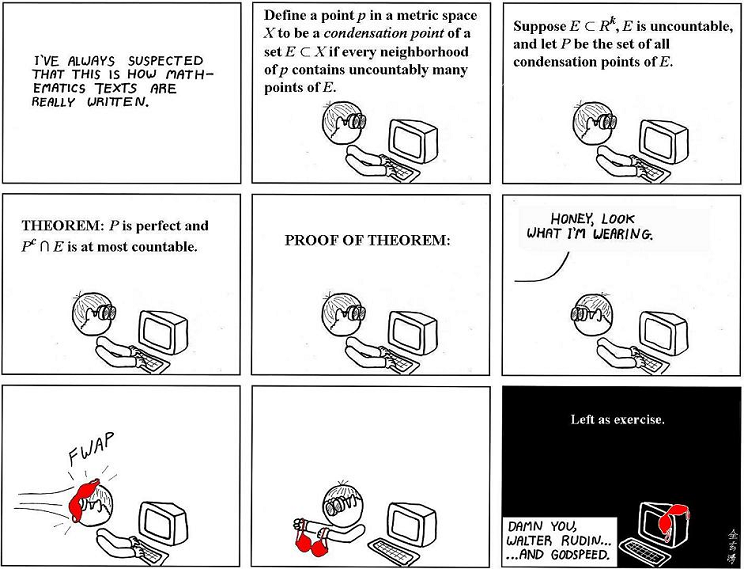
\includegraphics[width=14cm]{media/abstruse-goose-exercise.png}
	\\ \scriptsize Image from \cite{img:exercise}
\end{center}

% I personally find most exercises to not be that interesting, and I've tried to keep boring ones to a minimum.
% Regardless, I've tried hard to pick problems that are fun to think about and, when possible, to give them
% the kind of flavor you might find on the IMO or Putnam (even when the underlying background is different).

\section{Paper}
At the risk of being blunt,
\begin{moral}
Read this book with pencil and paper.
\end{moral}
Here's why:

\begin{center}
	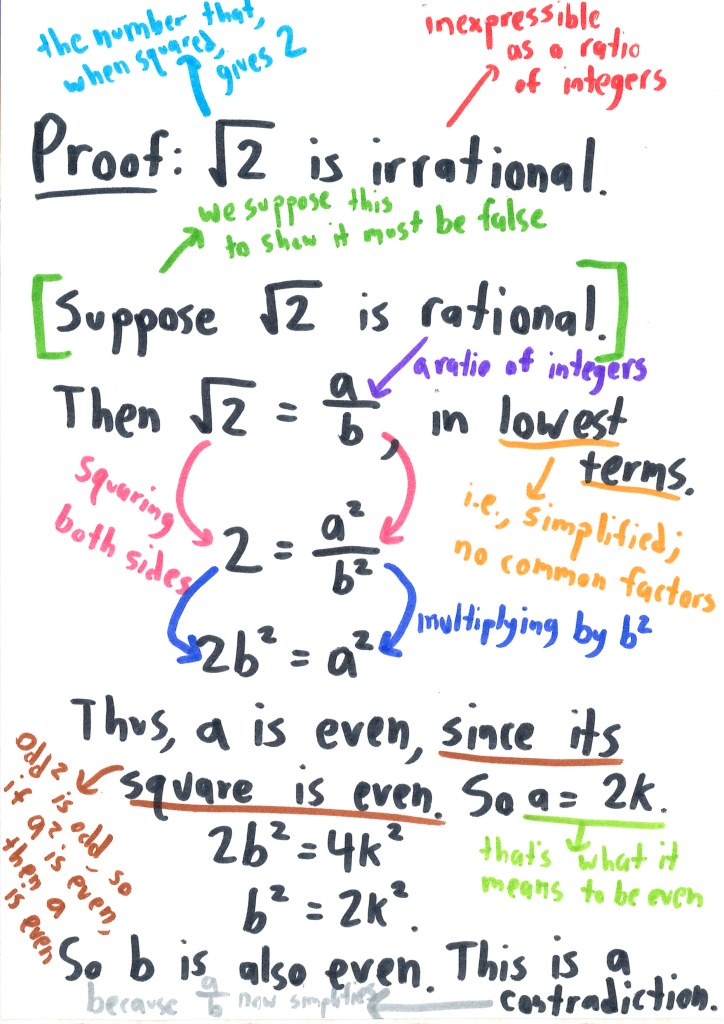
\includegraphics[width=0.5\textwidth]{media/read-with-pencil.jpg}
	\\ \scriptsize Image from \cite{img:read_with_pencil}
\end{center}
You are not God.
You cannot keep everything in your head.\footnote{See also
	\url{https://blog.evanchen.cc/2015/03/14/writing/} and the source above.}
If you've printed out a hard copy, then write in the margins.
If you're trying to save paper,
grab a notebook or something along with the ride.
Somehow, some way, make sure you can write. Thanks.

\section{On the importance of examples}
I am pathologically obsessed with examples.
In this book, I place all examples in large boxes to draw emphasis to them,
which leads to some pages of the book simply consisting of sequences of boxes
one after another. I hope the reader doesn't mind.

I also often highlight a ``prototypical example'' for some sections,
and reserve the color red for such a note.
The philosophy is that any time the reader sees a definition
or a theorem about such an object, they should test it
against the prototypical example.
If the example is a good prototype, it should be immediately clear
why this definition is intuitive, or why the theorem should be true,
or why the theorem is interesting, et cetera.

Let me tell you a secret.  Whenever I wrote a definition or a theorem in this book,
I would have to recall the exact statement from my (quite poor) memory.
So instead I often consider the prototypical example,
and then only after that do I remember what the definition or the theorem is.
Incidentally, this is also how I learned all the definitions in the first place.
I hope you'll find it useful as well.

\section{Conventions and notations}
This part describes some of the less familiar notations and definitions
and settles for once and for all some annoying issues
(``is zero a natural number?'').
Most of these are ``remarks for experts'':
if something doesn't make sense,
you probably don't have to worry about it for now.

A full glossary of notation used can be found in the appendix.

\subsection{Natural numbers are positive}
The set $\NN$ is the set of \emph{positive} integers, not including $0$.
In the set theory chapters, we use $\omega = \{0, 1, \dots\}$
instead, for consistency with the rest of the book.

\subsection{Sets and equivalence relations}
This is brief, intended as a reminder for experts.
Consult \Cref{ch:sets_functions} for full details.

An \vocab{equivalence relation} on a set $X$ is a relation $\sim$
which is symmetric, reflexive, and transitive.
An equivalence relation partitions $X$
into several \vocab{equivalence classes}.
We will denote this by $X / {\sim}$.
An element of such an equivalence class is a
\vocab{representative} of that equivalence class.

I always use $\cong$ for an ``isomorphism''-style relation
(formally: a relation which is an isomorphism in a reasonable category).
The only time $\simeq$ is used in the Napkin is for homotopic paths.

I generally use $\subseteq$ and $\subsetneq$ since these are non-ambiguous,
unlike $\subset$.  I only use $\subset$ on rare occasions in which equality
obviously does not hold yet pointing it out would be distracting.
For example, I write $\QQ \subset \RR$
since ``$\QQ \subsetneq \RR$'' is distracting.

I prefer $S \setminus T$ to $S - T$.

The power set of $S$ (i.e.,\ the set of subsets of $S$),
is denoted either by $2^S$ or $\mathcal P(S)$.

\subsection{Functions}
This is brief, intended as a reminder for experts.
Consult \Cref{ch:sets_functions} for full details.

Let $X \taking f Y$ be a function:
\begin{itemize}
\ii By $f\pre(T)$ I mean the \vocab{pre-image}
\[ f\pre(T) \defeq \left\{ x \in X \mid f(x) \in T \right\}.  \]
This is in contrast to the $f\inv(T)$ used in the rest of the world;
I only use $f\inv$ for an inverse \emph{function}.

By abuse of notation, we may abbreviate $f\pre(\{y\})$ to $f\pre(y)$.
We call $f\pre(y)$ a \vocab{fiber}.

\ii By $f\im(S)$ I mean the \vocab{image}
\[ f\im(S) \defeq \left\{ f(x) \mid x \in S \right\}. \]
Almost everyone else in the world uses $f(S)$
(though $f[S]$ sees some use, and $f''(S)$ is often used in logic)
but this is abuse of notation,
and I prefer $f\im(S)$ for emphasis.
This image notation is \emph{not} standard.

\ii If $S \subseteq X$, then the \vocab{restriction} of $f$ to $S$
is denoted $f \restrict{S}$,
i.e.\ it is the function $f \restrict{S} \colon S \to Y$.

\ii Sometimes functions $f \colon X \to Y$
are \emph{injective} or \emph{surjective};
I may emphasize this sometimes by writing
$f \colon X \injto Y$ or $f \colon X \surjto Y$, respectively.
\end{itemize}

\subsection{Cycle notation for permutations}
\label{subsec:cycle_notation}

Additionally, a permutation on a finite set may be denoted
in \emph{cycle notation},
as described in say \url{https://en.wikipedia.org/wiki/Permutation#Cycle_notation}.
For example the notation $(1 \; 2 \; 3 \; 4)(5 \; 6 \; 7)$
refers to the permutation with
$1 \mapsto 2$, $2 \mapsto 3$, $3 \mapsto 4$, $4 \mapsto 1$,
$5 \mapsto 6$, $6 \mapsto 7$, $7 \mapsto 5$.
Usage of this notation will usually be obvious from context.

\subsection{Rings}
All rings have a multiplicative identity $1$ unless otherwise specified.
We allow $0=1$ in general rings but not in integral domains.

\textbf{All rings are commutative unless otherwise specified.}
There is an elaborate scheme for naming rings which are not commutative,
used only in the chapter on cohomology rings:

\begin{center}
	\small
	\begin{tabular}[h]{|c|cc|}
		\hline
		& Graded & Not Graded \\ \hline
		$1$ not required & graded pseudo-ring & pseudo-ring \\
		Anticommutative, $1$ not required & anticommutative pseudo-ring & N/A \\
		Has $1$ & graded ring & N/A \\
		Anticommutative with $1$ & anticommutative ring & N/A \\
		Commutative with $1$ & commutative graded ring & ring \\ \hline
	\end{tabular}
\end{center}

On the other hand, an \emph{algebra} always has $1$,
but it need not be commutative.

\subsection{Choice}
We accept the Axiom of Choice, and use it freely.

\section{Further reading}
The appendix \Cref{ch:refs} contains a list of resources I like,
and explanations of pedagogical choices that I made for each chapter.
I encourage you to check it out.

In particular, this is where you should go for further reading!
There are some topics that should be covered in the Napkin,
but are not, due to my own ignorance or laziness.
The references provided in this appendix should hopefully help partially
atone for my omissions.


% I DON'T want to reset the page number for mainmatter,
% so save it to restore later
\cleardoublepage
\newcounter{temppage}
\setcounter{temppage}{\value{page}}
\mainmatter
\setcounter{page}{\value{temppage}}

\tableofcontents

\Opensolutionfile{tex/backmatter/all-hints}
\Opensolutionfile{tex/backmatter/all-solns}

\part{Starting Out}
\label{part:startout}
\parttoc
\setcounter{chapter}{-1} % sales pitch should be chapter 0
\chapter{Sales pitches}
\label{ch:sales}
\newcommand{\pitch}[1]{\ii[\textsf{\color{blue}\ref{#1}}.] \textsf{\color{blue} \textbf{\nameref{#1}.}} \\[1ex]} % for now. . .
\newcommand{\buzzword}[1]{\textbf{\color{green!40!black} #1}}

This chapter contains a pitch for each part,
to help you decide what you want to read
and to elaborate more on how they are interconnected.

For convenience, here is again the dependency plot
that appeared in the frontmatter.
%\chapter*{Graph of Chapter Dependencies}
%\addcontentsline{toc}{chapter}{Graph of Chapter Dependencies}

\bgroup
\renewcommand{\href}[1]{} % temp disable links
\hypersetup{linkcolor=black} % temporarily make internal refs black, so part labels are not all maroon
\renewcommand{\solidwidth}{0.7pt}
\renewcommand{\boldwidth}{1.5pt}

\setcounter{diagheight}{50}
\begin{chart}
\reqhalfcourse 20,45:{Ch \ref*{ch:group_intro},\ref*{ch:homomorphisms_quotient}-\ref*{ch:flavors_rings}}{\hyperref[part:absalg]{Abs Alg}}{}
\reqhalfcourse 55,45:{Ch \ref*{ch:metric_space},\ref*{ch:metric_properties}-\ref*{ch:compactness}}{\hyperref[part:basictop]{Topology}}{}
\halfcourse 33,45:{Ch \ref*{ch:vector_spaces}-\ref*{ch:duals_adjoint_transposes},\ref*{ch:PID_structure_theorem}}{\hyperref[part:linalg]{Lin Alg}}{}
\halfcourse 5,35:{Ch \ref*{ch:group_actions}}{\hyperref[part:groups]{Grp Act}}{}
\halfcourse 5,24:{Ch \ref*{ch:sylow}}{\hyperref[ch:sylow]{Grp Classif}}{}
\halfcourse 30,35:{Ch \ref*{ch:representations_of_algebras}-\ref*{ch:applications}}{\hyperref[part:repth]{Rep Th}}{}
\halfcourse 45,43:{Ch \ref*{ch:quantum_states_and_measurements}-\ref*{ch:shors_algorithm}}{\hyperref[part:quantum]{Quantum}}{}
\halfcourse 64,38:{Ch \ref*{ch:calc_limits}-\ref*{ch:riemann_integrals}}{\hyperref[part:calc]{Calc}}{}
\halfcourse 64,30:{Ch \ref*{ch:holomorphic_functions}-\ref*{ch:abel_ruffini_theorem}}{\hyperref[part:cmplxana]{Cmplx Ana}}{}
\halfcourse 55,20:{Ch \ref*{ch:measure_space}-\ref*{ch:pontryagin}}{\hyperref[part:measure]{Measure/Pr}}{}
\halfcourse 48,28:{Ch \ref*{ch:multivar_calculus}-\ref*{ch:line_bundles}}{\hyperref[part:diffgeo]{Diff Geo}}{}
\halfcourse 40,10:{Ch \ref*{ch:algebraic_integers}-\ref*{ch:galois_theory}}{\hyperref[part:algnt1]{Alg NT 1}}{}
\halfcourse 40,0:{Ch \ref*{ch:finite_fields}-\ref*{ch:artin_reciprocity}}{\hyperref[part:algnt2]{Alg NT 2}}{}
\halfcourse 23,10:{Ch \ref*{ch:top_constructions}-\ref*{ch:covering_projections}}{\hyperref[part:algtop1]{Alg Top 1}}{}
\halfcourse 20,28:{Ch \ref*{ch:cats}-\ref*{ch:abelian_categories}}{\hyperref[part:cats]{Cat Th}}{}
\halfcourse 23,0:{Ch \ref*{ch:singular_homology}-\ref*{ch:application_of_cohomology}}{\hyperref[part:algtop2]{Alg Top 2}}{}
\halfcourse 6,10:{Ch \ref*{ch:affine_varieties}-\ref*{ch:morphisms_of_varieties}}{\hyperref[part:ag1]{Alg Geo 1}}{}
\halfcourse 6,0:{Ch \ref*{ch:sheaves_and_ringed_spaces}-\ref*{ch:morphisms_of_locally_ringed_spaces}}{\hyperref[part:ag2]{Alg Geo 2-3}}{}
\reqhalfcourse 5,45:{Ch \ref*{ch:zorn}-\ref*{ch:break_CH}}{\hyperref[part:st1]{Set Theory}}{}

%% Basic alg ch
\prereqc 20,45,30,35;0:    % Abs Alg -> Rep Th
\coreqc  20,45,33,45;0:    % Abs Alg -> Lin Alg
\prereqc 33,45,30,35;0:    % Lin Alg -> Rep Th
\prereqc 33,45,45,43;0:    % Lin Alg -> Quantum
%% Category theory
\prereqc 20,45,20,28;0:    % Grp -> Cat Th
\coreqc  20,45,20,28;0:    % Abs Alg -> Cat Th
\coreqc  33,45,20,28;80:   % Lin Alg -> Cat Th
\coreqc  55,45,20,28;-40:  % Top -> Cat Th
\coreqc  20,28,30,35;0:    % Cat Th -> Rep Th
%% Group theory chain
\prereqc 20,45,5,35;0:     % Grp -> Grp Act
\prereqc  5,35,5,24;0:     % Grp Act -> Grp Class
%% Analysis chain
\prereqc 33,45,48,28;30:   % Lin Alg -> Diff Geo
\prereqc 55,45,64,38;0:    % Top -> Diff Geo
\coreqc  64,38,48,28;50:   % Calc -> Diff Geo
\prereqc 55,45,48,28;10:   % Top -> Diff Geo
\prereqc 55,45,64,38;0:    % Top -> Calc
\coreqc  64,38,64,30;0:    % Calc -> Cmplx Ana
\prereqc 55,45,64,30;-10:  % Top -> Cmplx Ana
\coreqc  23,10,64,30;0:    % AT1 -> Cmplx Ana
\prereqc 55,45,55,20;0:    % Top -> Meas/Pr
\coreqc  64,38,55,20;50:   % Calc -> Meas/Pr
%% Alg Geom
\prereqc 6,10,6,0;0:       % AG1 -> AG2
\prereqc 20,45,6,10;0:     % Abs Alg -> AG1
\prereqc 55,45,6,10;-40:   % Top -> AG1
\coreqc  20,28,6,10;0:     % Cat Th -> AG1
\prereqc 20,28,6,0;-18:    % Cat -> AG2
%% Alg Top
\prereqc 23,10,23,0;0:     % AT1 -> AT2
\prereqc 55,45,23,10;0:    % Top -> AT1
\prereqc  5,35,23,10;20:   % Grp Act -> AT1
\coreqc 23,10,20,28;20:    % AT1 -> Cat
\prereqc 20,28,23,0;-190:  % Cat -> AT2
%% Alg NT
\prereqc 40,10,40,0;0:     % ANT1 -> ANT2
\prereqc 20,45,40,10;-40:  % Abs Alg -> ANT1
\prereqc 33,45,40,10;50:   % Lin Alg -> ANT1
\prereqc  5,35,40,0;10:    % Grp Act -> ANT2
\end{chart}
\egroup


\section{The basics}
\begin{itemize}
\pitch{part:startout}
I made a design decision that the first part
should have a little bit of both algebra and topology:
so this first chapter begins by defining a \buzzword{group},
while the second chapter begins by defining a \buzzword{metric space}.
The intention is so that newcomers get to see two different
examples of ``sets with additional structure''
in somewhat different contexts,
and to have a minimal amount of literacy as these sorts
of definitions appear over and over.\footnote{In particular,
	I think it's easier to learn
	what a homeomorphism is after seeing group isomorphism,
	and what a homomorphism is after seeing continuous map.}

\pitch{part:absalg}
The algebraically inclined can then delve into
further types of algebraic structures:
some more details of \buzzword{groups},
and then \buzzword{rings} and \buzzword{fields} ---
which will let you generalize $\ZZ$, $\QQ$, $\RR$, $\CC$.
So you'll learn to become familiar with all sorts of other nouns
that appear in algebra, unlocking a whole host of objects
that one couldn't talk about before.

We'll also come to \buzzword{ideals},
which generalize the GCD in $\ZZ$ that you might know of.
For example, you know in $\ZZ$ that any integer
can be written in the form $3a+5b$ for $a,b \in \ZZ$,
since $\gcd(3,5)=1$.
We'll see that this statement is really
a statement of ideals: ``$(3,5)=1$ in $\ZZ$'',
and thus we'll understand in what situations
it can be generalized, e.g.\ to polynomials.

\pitch{part:basictop}
The more analytically inclined can instead move into topology,
learning more about spaces.
We'll find out that ``metric spaces'' are actually too specific,
and that it's better to work with \buzzword{topological spaces},
which are based on the so-called \buzzword{open sets}.
You'll then get to see the buddings of some geometrical ideals,
ending with the really great notion of \buzzword{compactness},
a powerful notion that makes real analysis tick.

One example of an application of compactness to tempt you now:
a continuous function $f \colon [0,1] \to \RR$
always achieves a \emph{maximum} value.
(In contrast, $f \colon (0,1) \to \RR$ by $x \mapsto 1/x$ does not.)
We'll see the reason is that $[0,1]$ is compact.
\end{itemize}

\section{Abstract algebra}
\begin{itemize}
\pitch{part:linalg}
In high school, linear algebra is often really unsatisfying.
You are given these arrays of numbers,
and they're manipulated in some ways that don't really make sense.
For example, the determinant is defined as this
funny-looking sum with a bunch of products that seems
to come out of thin air. Where does it come from?
Why does $\det(AB) = \det A \det B$ with such a bizarre formula?

Well, it turns out that you \emph{can} explain all of these things!
The trick is to not think of linear algebra
as the study of matrices,
but instead as the study of \emph{linear maps}.
In earlier chapters we saw that we got great generalizations
by speaking of ``sets with enriched structure'' and ``maps between them''.
This time, our sets are \buzzword{vector spaces}
and our maps are \buzzword{linear maps}.
We'll find out that a matrix is actually just
a way of writing down a linear map as an array of numbers,
but using the ``intrinsic'' definitions
we'll de-mystify all the strange formulas from high school
and show you where they all come from.

In particular, we'll see \emph{easy} proofs
that column rank equals row rank,
determinant is multiplicative, trace is the sum of the diagonal entries.
We'll see how the dot product works,
and learn all the words starting with ``eigen-''.
We'll even have a bonus chapter for Fourier analysis
showing that you can also explain all the big buzz-words
by just being comfortable with vector spaces.

\pitch{part:groups}
Some of you might be interested in more about groups,
and this chapter will give you a way to play further.
It starts with an exploration of \buzzword{group actions},
then goes into a bit on \buzzword{Sylow theorems},
which are the tools that let us try to \emph{classify all groups}.

\pitch{part:repth}
If $G$ is a group, we can try to understand
it by implementing it as a \emph{matrix},
i.e.\ considering embeddings $G \injto \GL_n(\CC)$.
These are called \buzzword{representations} of $G$;
it turns out that they can be decomposed into \buzzword{irreducible} ones.
Astonishingly we will find that we can
\emph{basically characterize all of them}:
the results turn out to be short and completely unexpected.

For example, we will find out that there are finitely
many irreducible representations of a given finite group $G$;
if we label them $V_1$, $V_2$, \dots, $V_r$,
then we will find that $r$ is the number
of conjugacy classes of $G$, and moreover that
\[ |G| = (\dim V_1)^2 + \dots + (\dim V_r)^2 \]
which comes out of nowhere!

The last chapter of this part will show you some
unexpected corollaries.
Here is one of them:
let $G$ be a finite group and create variables $x_g$
for each $g \in G$.
A $|G| \times |G|$ matrix $M$ is defined by setting
the $(g,h)$th entry to be the variable $x_{g \cdot h}$.
Then this determinant will turn out to \emph{factor},
and the factors will correspond to the $V_i$ we described above:
there will be an irreducible factor of degree $\dim V_i$
appearing $\dim V_i$ times.
This result, called the \buzzword{Frobenius determinant},
is said to have given birth to representation theory.

\pitch{part:quantum}
If you ever wondered what \buzzword{Shor's algorithm} is,
this chapter will use the built-up linear algebra to tell you!
\end{itemize}

\section{Real and complex analysis}
\begin{itemize}
\pitch{part:calc}
In this part, we'll use our built-up knowledge of
metric and topological spaces to give short, rigorous definitions
and theorems typical of high school calculus.
That is, we'll really define and prove most everything you've seen about
\buzzword{limits}, \buzzword{series}, \buzzword{derivatives}, and \buzzword{integrals}.

Although this might seem intimidating,
it turns out that actually, by the time we start this chapter,
\emph{the hard work has already been done}:
the notion of limits, open sets, and compactness
will make short work of what was swept under the rug in AP calculus.
Most of the proofs will thus actually be quite short.
We sit back and watch all the pieces slowly come together
as a reward for our careful study of topology beforehand.

That said, if you are willing to suspend belief,
you can actually read most of the other parts
without knowing the exact details of all the calculus here,
so in some sense this part is ``optional''.

\pitch{part:cmplxana}
It turns out that \buzzword{holomorphic functions}
(complex-differentiable functions)
are close to the nicest things ever:
they turn out to be given by a Taylor series
(i.e.\ are basically polynomials).
This means we'll be able to prove unreasonably nice results
about holomorphic functions $\CC \to \CC$, like
\begin{itemize}
	\ii they are determined by just a few inputs,
	\ii their contour integrals are all zero,
	\ii they can't be bounded unless they are constant,
	\ii \dots.
\end{itemize}
We then introduce \buzzword{meromorphic functions},
which are like quotients of holomorphic functions,
and find that we can detect their zeros by simply drawing
loops in the plane and integrating over them:
the famous \buzzword{residue theorem} appears.
(In the practice problems, you will see this even gives
us a way to evaluate real integrals that can't be evaluated otherwise.)

\pitch{part:measure}
Measure theory is the upgraded version of integration.
The Riemann integration is for a lot of purposes not really sufficient;
for example, if $f$ is the function equals $1$ at rational numbers
but $0$ at irrational numbers,
we would hope that $\int_0^1 f(x) \; dx = 0$,
but the Riemann integral is not capable of handling this function $f$.

The \buzzword{Lebesgue integral} will handle these mistakes
by assigning a \emph{measure} to a generic space $\Omega$,
making it into a \buzzword{measure space}.
This will let us develop a richer theory of integration
where the above integral \emph{does} work out to zero
because the ``rational numbers have measure zero''.
Even the development of the measure will be an achievement,
because it means we've developed a rigorous, complete way
of talking about what notions like area and volume mean ---
on any space, not just $\RR^n$!
So for example the Lebesgue integral will let us
integrate functions over any \buzzword{measure space}.

\pitch{part:prob}
Using the tools of measure theory, we'll be able to start
giving rigorous definitions of \buzzword{probability}, too.
We'll see that a \buzzword{random variable} is actually
a function from a measure space of worlds to $\RR$,
giving us a rigorous way to talk about its probabilities.
We can then start actually stating results like
the \buzzword{law of large numbers} and \buzzword{central limit theorem}
in ways that make them both easy to state and straightforward to prove.

\pitch{part:diffgeo}
Multivariable calculus is often confusing
because of all the partial derivatives.
But we'll find out that, armed with our good understanding
of linear algebra, that we're really looking at a \buzzword{total derivative}:
at every point of a function $f \colon \RR^n \to \RR$
we can associate a \emph{linear map} $Df$ which
captures in one object the notion of partial derivatives.
Set up this way, we'll get to see versions of \buzzword{differential forms}
and \buzzword{Stokes' theorem},
and we finally will know what the notation $dx$ really means.
In the end, we'll say a little bit about manifolds in general.
\end{itemize}

\section{Algebraic number theory}
\begin{itemize}
\pitch{part:algnt1}
Why is $3+\sqrt5$ the conjugate of $3-\sqrt5$?
How come the norm $\norm{a+b\sqrt5} = a^2-5b^2$ used in Pell's equations
just happens to be multiplicative?
Why is it we can do factoring into primes in $\ZZ[i]$
but not in $\ZZ[\sqrt{-5}]$?
All these questions and more will be answered in this part,
when we learn about \buzzword{number fields},
a generalization of $\QQ$ and $\ZZ$ to things like $\QQ(\sqrt5)$
and $\ZZ[\sqrt{5}]$.
We'll find out that we have unique factorization into prime ideals,
that there is a real \emph{multiplicative norm} in play here,
and so on.
We'll also see that Pell's equation falls out of this theory.

\pitch{part:algnt2}
All the big buzz-words come out now:
\buzzword{Galois groups}, the \buzzword{Frobenius}, and friends.
We'll see quadratic reciprocity is just a shadow of
the behavior of the Frobenius element,
and meet the \buzzword{Chebotarev density theorem},
which generalizes greatly the Dirichlet theorem on the infinitude
of primes which are $a \pmod n$.
Towards the end, we'll also state \buzzword{Artin reciprocity},
one of the great results of \buzzword{class field theory},
and how it generalizes quadratic reciprocity and cubic reciprocity.
\end{itemize}

\section{Algebraic topology}
\begin{itemize}
\pitch{part:algtop1}
What's the difference between an annulus and disk?
Well, one of them has a ``hole'' in it,
but if we are just given intrinsic topological spaces
it's hard to make this notion precise.
The \buzzword{fundamental group} $\pi_1(X)$
and more general \buzzword{homotopy group}
will make this precise --- we'll find a way to define an abelian group
$\pi_1(X)$ for every topological space $X$ which captures the idea
there is a hole in the space, by throwing lassos into the space
and seeing if we can reel them in.

Amazingly, the fundamental group $\pi_1(X)$ will, under mild conditions,
tell you about ways to cover $X$ with a so-called
\buzzword{covering projection}.
One picture is that one can wrap a real line $\RR$ into a helix shape
and then project it down into the circle $S^1$.
This will turn out to correspond to the fact that $\pi_1(S^1) = \ZZ$
which has only one subgroup.
More generally the subgroups of $\pi_1(X)$ will be in
bijection with ways to cover the space $X$!

\pitch{part:cats}
What do fields, groups, manifolds, metric spaces, measure spaces,
modules, representations, rings, topological spaces, vector spaces,
all have in common?
Answer: they are all ``objects with additional structure'',
with maps between them.

The notion of \buzzword{category} will appropriately generalize all of them.
We'll see that all sorts of constructions and ideas
can be abstracted into the framework of a category,
in which we \emph{only} think about objects and arrows between them,
without probing too hard into the details of what those objects are.
This results in drawing many \buzzword{commutative diagrams}.

For example, any way of taking an object in one category
and getting another one (for example $\pi_1$ as above,
from the category of spaces into the category of groups)
will probably be a \buzzword{functor}.
We'll unify $G \times H$, $X \times Y$, $R \times S$,
and anything with the $\times$ symbol into the notion of a product,
and then even more generally into a \buzzword{limit}.
Towards the end, we talk about \buzzword{abelian categories}
and talk about the famous
\buzzword{snake lemma}, \buzzword{five lemma}, and so on.

\pitch{part:algtop2}
Using the language of category theory,
we then resume our adventures in algebraic topology,
in which we define the \buzzword{homology groups}
which give a different way of noticing holes in a space,
in a way that is longer to define but easier to compute in practice.
We'll then reverse the construction to get so-called
\buzzword{cohomology rings} instead,
which give us an even finer invariant for telling spaces apart.
\end{itemize}

\section{Algebraic geometry}
\begin{itemize}
\pitch{part:ag1}
We begin with a classical study of classical \buzzword{complex varieties}:
the study of intersections of polynomial equations over $\CC$.
This will naturally lead us into the geometry of rings,
giving ways to draw pictures of ideals,
and motivating \buzzword{Hilbert's nullstellensatz}.
The \buzzword{Zariski topology} will show its face,
and then we'll play with \buzzword{projective varieties}
and \buzzword{quasi-projective varieties},
with a bonus detour into \buzzword{B\'{e}zout's theorem}.
All this prepares us for our journey into schemes.

\pitch{part:ag2}
We now get serious and delve into Grothendieck's definition of
an \buzzword{affine scheme}:
a generalization of our classical varieties
that allows us to start with any ring $A$
and construct a space $\Spec A$ on it.
We'll equip it with its own Zariski topology
and then a sheaf of functions on it,
making it into a \buzzword{locally ringed space};
we will find that the sheaf can be understood
effectively in terms of \buzzword{localization} on it.
We'll find that the language of commutative algebra provides
elegant generalizations of what's going on geometrically:
prime ideals correspond to irreducible closed subsets,
radical ideals correspond to closed subsets,
maximal ideals correspond to closed points, and so on.
We'll draw lots of pictures of spaces and examples to accompany this.
\end{itemize}

\section{Set theory}
\begin{itemize}
\pitch{part:st1}
Why is \buzzword{Russell's paradox} such a big deal
and how is it resolved?
What is this \buzzword{Zorn's lemma}
that everyone keeps talking about?
In this part we'll learn the answers to these questions
by giving a real description of the \buzzword{Zermelo-Frankel}
axioms, and the \buzzword{axiom of choice},
delving into the details of how math is built axiomatically
at the very bottom foundations.
We'll meet the \buzzword{ordinal numbers} and \buzzword{cardinal numbers}
and learn how to do \buzzword{transfinite induction} with them.

\pitch{part:st2}
The \buzzword{continuum hypothesis}
states that there are no cardinalities
between the size of the natural numbers and the size of the real numbers.
It was shown to be \emph{independent} of the axioms ---
one cannot prove or disprove it.
How could a result like that possibly be proved?
Using our understanding of the ZF axioms,
we'll develop a bit of \buzzword{model theory}
and then use \buzzword{forcing} in order to show
how to construct entire models of the universe
in which the continuum hypothesis is true or false.
\end{itemize}

\chapter{Sets}
\label{ch:sets}

\section{What do we know about sets so far?}

If we are to believe Wikipedia blindly, then
\begin{quote}
	In mathematics, a set is a collection of different things; these things are called elements or members of the set and are typically mathematical objects of any kind: numbers, symbols, points in space, lines, other geometrical shapes, variables, or even other sets.
\end{quote}

\begin{example}
	[Famous sets]
	Some sets you must have seen by now:
	\begin{enumerate}
	\item Natural Numbers: $\NN$
	\item Integers: $\ZZ$
	\item Rational Numbers: $\QQ$
	\item Real Numbers: $\RR$
	\item Complex Numbers: $\CC$
	\end{enumerate}
\end{example}

\begin{abuse}
	We have progressed from the age of Bhimbetka. So no proof by pictures, Venn diagrams, or any other form of
	doodling. You are however encouraged to draw pictures to gain intuition.
\end{abuse}

Assuming one has done high school mathematics or gone through the required \hyperref[ch:sets_functions]{notation to be followed}, we will refresh our set theory basics with a couple of exercises

\section{\problemhead}

\begin{problem}
	 Define the symmetric difference between two sets as $A \Delta B \triangleq(A \backslash B) \cup(B \backslash A)$. Show that:
	 \begin{enumerate}[a)]
		\item $A \Delta B=(A \cup B) \backslash(A \cap B)$.
		\item $A \backslash(A \Delta B)=A \cap B$.
	\end{enumerate}
	\begin{hint}
		Tbdl
	\end{hint}
	\begin{sol}
		Tbdl
	\end{sol}
\end{problem}

\begin{problem}
	If $A \subseteq B$ and $C \subseteq D$, then prove that $(A \cap C) \cup(B \cap D)=B \cap D$.
\end{problem}

\begin{problem}
	Let $I$ be any set, and consider the collection of sets $\left\{A_{i}: i \in I\right\}$. Show that for any other set $B, B \cap\left(\cap_{i \in I} A_{i}\right)=\cap \cap_{i \in I}\left(B \cap A_{i}\right)$. Hence prove $B \backslash \cup_{i \in I} A_{i}=\cap_{i \in I}\left(B \backslash A_{i}\right)$.
\end{problem}

\begin{problem}
	Prove the following:
	\begin{enumerate}[a)]
	\item $\cap_{n=1}^{\infty}\left(-\frac{1}{n}, \frac{1}{n}\right)=\{0\}$.
	\item $\cap_{n=1}^{\infty}\left[1-\frac{1}{n}, \infty\right)=[1, \infty)$.
	\end{enumerate}
\end{problem}

\begin{problem}
	Consider the function $f: X \rightarrow Y$, and let $A \subseteq X$ and $B \subseteq Y$. Define the generalised inverse of $f$ by $f^{-1}(B)=\{x \in$ $X: f(x) \in B\}$. Also, define $f(A)=\{y \in Y: \exists x \in A$ such that $f(x)=y\}$.
	\begin{enumerate}[a)]
	\item Show that $f^{-1}\left(B_{1} \cup B_{2}\right)=f^{-1}\left(B_{1}\right) \cup f^{-1}\left(B_{2}\right), \forall B_{1}, B_{2} \subseteq Y$.
	\item Show that $f^{-1}\left(B_{1} \cap B_{2}\right)=f^{-1}\left(B_{1}\right) \cap f^{-1}\left(B_{2}\right), \forall B_{1}, B_{2} \subseteq Y$.
	\item Show that $A \subseteq f^{-1}(f(A))$. Give an example to show that the inclusion can be strict.
	\item Show that $f\left(f^{-1}(B)\right) \subseteq B$. Show that equality holds if $f$ is surjective.
	\end{enumerate}
\end{problem}

\begin{problem}
	Consider a function $f: \mathbb{R}^{n} \rightarrow \mathbb{R}^{n}$. Let $A_{i} \subseteq \mathbb{R}, 1 \leq i \leq n$.
	\begin{enumerate}[a)]
	\item Show that $f\left(\times_{i=1}^{n} A_{i}\right) \subseteq f\left(A_{1} \times \mathbb{R} \times \ldots \times \mathbb{R}\right) \cap f\left(\mathbb{R} \times A_{2} \times \ldots \times \mathbb{R}\right) \cap \ldots \cap f\left(\mathbb{R} \times \mathbb{R} \times \ldots \times A_{n}\right)$.
	\item Provide an example to show that the inclusion can be strict.
	\end{enumerate}
\end{problem}

\begin{problem}[Final boss: Bradley, if you happen to be a Fullmetal Alchemist fan]
	Define the set $T_{n} \triangleq \cup_{i=0}^{n-1}\left[\frac{i}{n}, \frac{i+1}{n}\right] \times\left[0,1-\frac{i}{n}\right]$. Show that $\cap_{n \in \mathbb{N}} T_{n}=\left\{(x, y) \in \mathbb{R}^{2}: x+y \leq 1, x \geq 0, y \geq 0\right\}$.
\end{problem}

\part{Measure Theory}
\label{part:measure}
\parttoc

\part{Welcome to Calculus}
\label{part:calc}
\parttoc

\part{Appendix}
\parttoc
\appendix
% \automark{chapter} % change to chapter in appendix

\Closesolutionfile{tex/backmatter/all-hints}
\Closesolutionfile{tex/backmatter/all-solns}
\chapter{Pedagogical comments and references}
\label{ch:refs}
Here are some higher-level comments on the way specific topics were presented,
as well as pointers to further reading.

\section{Basic algebra and topology}
\subsection{Linear algebra and multivariable calculus}
Following the comments in \Cref{sec:basis_evil},
I dislike most presentations of linear algebra and multivariable calculus
since they miss the two key ideas, namely:
\begin{itemize}
	\ii In linear algebra, we study \emph{linear maps} between spaces.
	\ii In calculus, we \emph{approximate functions at points by linear functions}.
\end{itemize}
Thus, I believe linear algebra should
\emph{always} be taught before multivariable calculus.
In particular, I do not recommend most linear algebra or
multivariable calculus books.

For linear algebra, I've heard that \cite{ref:axler} follows this approach,
hence the appropriate name ``Linear Algebra Done Right''.
I followed with heavy modifications the proceedings of Math 55a,
see \cite{ref:55a}.

For multivariable calculus and differential geometry,
I found the notes \cite{ref:manifolds} to be unusually well-written.
I referred to it frequently while I was enrolled in Math 55b \cite{ref:55b}.

\subsection{General topology}
My personal view on spaces is that every space I ever work with
is either metrizable or is the Zariski topology.

I adopted the approach of \cite{ref:pugh}, using metric topology first.
I find that metric spaces are far more intuitive, and are a much better
way to get a picture of what open / closed / compact etc.\ sets look like.
This is the approach history took;
general topology grew out of metric topology.

I personally dislike starting any general topology class
by defining what a general topological space is,
because it doesn't communicate a good picture of open and closed sets
to draw pictures of.

\subsection{Groups and commutative algebra}
I teach groups before commutative rings but might convert later.
Rings have better examples, don't have the confusion of multiplicative
notation for additive groups, and modding out by ideals is more intuitive.

There's a specific thing I have a qualm with in group theory:
the way that the concept of a normal subgroup is introduced.
Only \cite{ref:gowers} does something similar to what I do.
Most other people simply \emph{define} a normal subgroup $N$
as one with $gNg\inv$ and then proceed to define modding out,
without taking the time to explain where this definition comes from.
I remember distinctly this concept as the first time in learning math
where I didn't understand what was going on.
Only in hindsight do I see where this definition came from;
I tried hard to make sure my own presentation didn't have this issue.

I deliberately don't include a chapter on just commutative algebra;
other than the chapter on rings and ideals.
The reason is that I always found it easier to learn
commutative algebra theorems on the fly,
in the context of something like algebraic number theory or algebraic geometry.
For example, I finally understand why radicals and the Nullstellensatz were important
when I saw how they were used in algebraic geometry.
Before then, I never understood why I cared about them.

\subsection{Calculus}
I do real analysis by using metric and general topology
as the main ingredient, since I think it's the most useful
later on and the most enlightening.
In some senses, I am still following \cite{ref:pugh}.

\section{Second-year topics}
\subsection{Measure theory and probability}
The main inspiration for these lectures is
Vadim Gorin's 18.175 at MIT;
\cite{ref:gorin} has really nice lecture notes taken by Tony Zhang.
I go into a bit more details of the measure theory,
and (for now) less into the probability.
But I think probability is a great way to motivate measure theory anyways,
and conversely, it's the right setting in to which state things like
the central limit theorem.

I also found \cite{ref:lebesgue} quite helpful,
as another possible reference.

\subsection{Complex analysis}
I picked the approach of presenting the Cauchy-Goursat theorem as given
(rather than proving a weaker version by Stokes' theorem, or whatever),
and then deriving the key result that holomorphic functions are analytic
from it.
I think this most closely mirrors the ``real-life'' use of complex
analysis, i.e.\ the computation of contour integrals.

The main reference for this chapter was \cite{ref:dartmouth}, which I recommend.

\subsection{Category theory}
I enthusiastically recommend \cite{ref:msci},
from which my chapters are based,
and which contains much more than I had time to cover.

You might try reading chapters {2-4} in reverse order though:
I found that limits were much more intuitive than adjoints.
But your mileage may vary.

The category theory will make more sense as you learn
more examples of structures: it will help to have read,
say, the chapters on groups, rings, and modules.

\subsection{Quantum algorithms}
The exposition given here is based off a full semester
at MIT taught by Seth Lloyd, in 18.435J \cite{ref:18-435}.
It is written in a far more mathematical perspective.

I only deal with finite-dimensional Hilbert spaces,
because that is all that is needed for Shor's algorithm,
which is the point of this chapter.
This is not an exposition intended for someone who wishes to seriously
study quantum mechanics (though it might be a reasonable first read):
the main purpose is to give students a little appreciation for
what this ``Shor's algorithm'' that everyone keeps talking about is.

\subsection{Representation theory}
I staunchly support teaching the representation of algebras first,
and then specializing to the case of groups by looking at $k[G]$.
The primary influence for the chapters here is \cite{ref:etingof},
and you might think of what I have here as just some selections
from the first four chapters of this source.

\subsection{Set theory}
Set theory is far off the beaten path.
The notes I have written are based off the class
I took at Harvard College, Math 145a \cite{ref:145a}.

My general impression is that the way I present set theory
(trying to remain intuitive and informal in a logical minefield)
is not standard. Possible other reference: \cite{ref:miquel}.

\section{Advanced topics}
\subsection{Algebraic topology}
I cover the fundamental group $\pi_1$ first, because I think the subject is more
intuitive this way. A possible reference in this topic is \cite{ref:munkres}.
Only later do I do the much more involved homology groups.
The famous standard reference for algebraic topology is \cite{ref:hatcher},
which is what almost everyone uses these days.
But I also found \cite{ref:maxim752} to be very helpful,
particularly in the part about cohomology rings.

I don't actually do very much algebraic topology.
In particular, I think the main reason to learn algebraic topology
is to see the construction of the homology and cohomology groups
from the chain complex, and watch the long exact sequence in action.
The concept of a (co)chain complex comes up often in other contexts as well,
like the cohomology of sheaves or Galois cohomology.
Algebraic topology is by far the most natural one.

I use category theory extensively, being a category-lover.

\subsection{Algebraic number theory}
I learned from \cite{ref:oggier_NT},
using \cite{ref:lenstra_chebotarev}
for the part about the Chebotarev density theorem.

When possible I try to keep the algebraic number theory chapter close at
heart to an ``olympiad spirit''.
Factoring in rings like $\ZZ[i]$ and $\ZZ[\sqrt{-5}]$
is very much an olympiad-flavored topic at heart:
one is led naturally to the idea of factoring in general rings of integers,
around which the presentation is built.
As a reward for the entire buildup, the exposition finishes
with the application of the Chebotarev density theorem to IMO 2003, Problem 6.

\subsection{Algebraic geometry}
My preferred introduction to algebraic geometry is \cite{ref:gathmann}
for a first read and \cite{ref:vakil} for the serious version.
Both sets of lecture notes are essentially self-contained.

I would like to confess now that I know relatively little algebraic geometry,
and in my personal opinion the parts on algebraic geometry
are the weakest part of the Napkin.
This is reflected in my work here:
in the entire set of notes I only barely finish defining a scheme,
the first central definition of the subject.

Nonetheless, I will foolishly still make some remarks about my own studies.
I think there are three main approaches to beginning the study of schemes:
\begin{itemize}
	\ii Only looking at affine and projective varieties,
	as part of an ``introductory'' class,
	typically an undergraduate course.
	\ii Studying affine and projective varieties closely
	and using them as the motivating example of a \emph{scheme},
	and then developing algebraic geometry from there.
	\ii Jumping straight into the definition of a scheme,
	as in the well-respected and challenging \cite{ref:vakil}.
\end{itemize}
I have gone with the second approach,
I think that if you don't know what a scheme is,
then you haven't learned algebraic geometry.
But on the other hand I think the definition of a scheme is
difficult to digest without having a good handle first on varieties.

These opinions are based on my personal experience of having
tried to learn the subject through all
three approaches over a period of a year.
Your mileage may vary.

I made the decision to, at least for the second part,
focus mostly on \emph{affine} schemes.
These already generalize varieties in several ways,
and I think the jump is too much if one starts
then gluing schemes together.
I would rather that the student first feel like
they really understand how an affine scheme works,
before going on into the world where they now have a general scheme $X$
which is locally affine (but probably not itself affine).
The entire chapter dedicated to a gazillion examples
of affine schemes is a hint of this.

\subsection{Riemann surfaces}
My friend recommends \cite{ref:miranda}. The preface of the book reads as follows:
\begin{quote}
	But I try to stress that the main examples
	(from the point of view of algebraic geometry) come from projective curves,
	and slowly but surely the text evolves to the algebraic category,
	culminating in an algebraic proof of the Riemann-Roch theorem.
	After returning to the analytic side of things for Abel's theorem,
	the progression is repeated again when sheaves and cohomology are discussed:
	first the analytic, then the algebraic category.
\end{quote}
Thus you can also use this as a resource to learn algebraic geometry.

Occasionally, a few concepts are not very well-motivated, such as divisors,
complex structure induced on plane curves, or line bundles.
In these cases, we try to explain the motivation clearly in the Napkin.

\section{Topics not in Napkin}
\subsection{Analytic number theory}
I never had time to write up notes in Napkin for these.
If you're interested though, I recommend \cite{ref:analytic_NT}.
They are highly accessible and delightful to read.
The only real prerequisites are a good handle on Cauchy's residue formula.

\chapter{Hints to selected problems}
\label{app:hints}
\begin{enumerate}
	\input{tex/backmatter/all-hints.out}
\end{enumerate}

\chapter{Sketches of selected solutions}
\label{app:sol}
\begin{enumerate}
	\input{tex/backmatter/all-solns.out}
\end{enumerate}


\chapter{Glossary of notations}
\section{General}
\begin{itemize}
	\ii $\forall$: for all
	\ii $\exists$: there exists
	\ii $\sign(\sigma)$: sign of permutation $\sigma$
	\ii $X \implies Y$: $X$ implies $Y$
\end{itemize}
\section{Functions and sets}
\begin{itemize}
	\ii $f\im(S)$ is the image of $f \colon X \to Y$ for $S \subseteq X$.
	\ii $f\inv(y)$ is the inverse for $f \colon X \to Y$ when $y \in Y$.
	\ii $f\pre(T)$ is the pre-image for $f \colon X \to Y$ when $T \subseteq Y$.
	\ii $f \restrict{S}$ is the restriction of $f \colon X \to Y$ to $S \subseteq X$.
	\ii $f^n$ is the function $f$ applied $n$ times
\end{itemize}

Below are some common sets.
These may also be thought of as groups,
rings, fields etc.\ in the obvious way.
\begin{itemize}
	\ii $\CC$: set of complex numbers
	\ii $\RR$: set of real numbers
	\ii $\NN$: set of positive integers
	\ii $\QQ$: set of rational numbers
	\ii $\ZZ$: set of integers
	\ii $\varnothing$: empty set
\end{itemize}

Some common notation with sets:
\begin{itemize}
	\ii $A \subset B$: $A$ is any subset of $B$
	\ii $A \subseteq B$: $A$ is any subset of $B$
	\ii $A \subsetneq B$: $A$ is a \emph{proper} subset of $B$
	\ii $S \times T$: Cartesian product of sets $S$ and $T$
	\ii $S \setminus T$: difference of sets $S$ and $T$
	\ii $S \cup T$: set union of $S$ and $T$
	\ii $S \cap T$: set intersection of $S$ and $T$
	\ii $S \sqcup T$: disjoint union of $S$ and $T$
	\ii $\left\lvert S \right\rvert$: cardinality of $S$
	\ii $S / {\sim}$: if $\sim$ is an equivalence relation on $S$,
	this is the set of equivalence classes
	\ii $x + S$: denotes the set $\{x+s \mid s \in S\}$.
	\ii $xS$: denotes the set $\{xs \mid s \in S\}$.
\end{itemize}

\section{Abstract and linear algebra}
Some common groups/rings/fields:
\begin{itemize}
	\ii $\Zc n$: cyclic group of order $n$
	\ii $\Zm n$: set of units of $\Zc n$.
	\ii $S_n$: symmetric group on $\{1, \dots, n\}$
	\ii $D_{2n}$: dihedral group of order $2n$.
	\ii $0$, $1$: trivial group (depending on context)
	\ii $\FF_p$: integers modulo $p$
\end{itemize}
Notation with groups:
\begin{itemize}
	\ii $1_G$: identity element of the group $G$
	\ii $N \normalin G$: subgroup $N$ is normal in $G$.
	\ii $G/N$: quotient group of $G$ by the normal subgroup $N$
	\ii $Z(G)$: center of group $G$
	\ii $N_G(H)$: normalizer of the subgroup $H$ of $G$
	\ii $G \times H$: product group of $G$ and $H$
	\ii $G \oplus H$: also product group,
	but often used when $G$ and $H$ are abelian
	(and hence we can think of them as $\ZZ$-modules)
	\ii $\Stab_G(x)$: the stabilizer of $x \in X$, if $X$ is acted on by $G$
	\ii $\FixPt g$, the set of fixed points by $g \in G$ (under a group action)
\end{itemize}
Notation with rings:
\begin{itemize}
	\ii $R/I$: quotient of ring $R$ by ideal $I$
	\ii $(a_1, \dots, a_n)$: ideal generated by the $a_i$
	\ii $R^\times$: the group of units of $R$
	\ii $R[x_1, \dots, x_n]$: polynomial ring in $x_i$,
	or ring obtained by adjoining the $x_i$ to $R$
	\ii $F(x_1, \dots, x_n)$: field obtained by adjoining $x_i$ to $F$
	\ii $R^d$: $d$th graded part of a graded (pseudo)ring $R$
\end{itemize}
Linear algebra:
\begin{itemize}
	\ii $\id$: the identity matrix
	\ii $V \oplus W$: direct sum
	\ii $V^{\oplus n}$: direct sum of $V$, $n$ times
	\ii $V \otimes W$: tensor product
	\ii $V^{\otimes n}$: tensor product of $V$, $n$ times
	\ii $V^\vee$: dual space
	\ii $T^\vee$: dual map (for $T$ a vector space)
	\ii $T^\dagger$: conjugate transpose (for $T$ a vector space)
	\ii $\left< -,-\right>$: a bilinear form
	\ii $\Mat(V)$: endomorphisms of $V$, i.e.\ $\Hom_k(V,V)$
	\ii $\ee_1$, \dots, $\ee_n$: the ``standard basis'' of $k^{\oplus n}$
\end{itemize}
\section{Quantum computation}
\begin{itemize}
	\ii $\ket{\psi}$: a vector in some vector space $H$
	\ii $\bra{\psi}$: a vector in some vector space $H^\vee$, dual to $\ket{\psi}$.
	\ii $\braket{\phi|\psi}$: evaluation of an element $\bra{\phi} \in H^\vee$ at $\ket{\phi} \in H$.
	\ii $\zup$, $\zdown$: spin $z$-up, spin $z$-down
	\ii $\xup$, $\xdown$: spin $x$-up, spin $x$-down
	\ii $\yup$, $\ydown$: spin $y$-up, spin $y$-down
\end{itemize}

\section{Topology and real/complex analysis}
Common topological spaces:
\begin{itemize}
	\ii $S^1$: the unit circle
	\ii $S^n$: surface of an $n$-sphere (in $\RR^{n+1}$)
	\ii $D^{n+1}$: closed $n+1$ dimensional ball (in $\RR^{n+1}$)
	\ii $\RP^n$: real projective $n$-space
	\ii $\CP^n$: complex projective $n$-space
\end{itemize}
Some topological notation:
\begin{itemize}
	\ii $\partial Y$: boundary of a set $Y$ (in some topological space)
	\ii $X/S$: quotient topology of $X$ by $S \subseteq X$
	\ii $X \times Y$: product topology of spaces $X$ and $Y$
	\ii $X \amalg Y$: disjoint union of spaces $X$ and $Y$
	\ii $X \vee Y$: wedge product of (pointed) spaces $X$ and $Y$
\end{itemize}
Real analysis (calculus 101):
\begin{itemize}
	\ii $\liminf$: limit infimum
	\ii $\limsup$: limit supremum
	\ii $\inf$: infimum
	\ii $\sup$: supremum
	\ii $\ZZ_p$: $p$-adic integers
	\ii $\QQ_p$: $p$-adic numbers
	\ii $f'$: derivative of $f$
	\ii $\int_a^b f(x) \; dx$: Riemann integral of $f$ on $[a,b]$
\end{itemize}
Complex analysis:
\begin{itemize}
	\ii $\int_\alpha f \; dz$: contour integral of $f$ along path $\alpha$
	\ii $\Res(f;p)$: the residue of a meromorphic function $f$ at point $p$
	\ii $\Wind(\gamma, p)$: winding number of $\gamma$ around $p$.
\end{itemize}
\section{Measure theory and probability}
\begin{itemize}
	\ii $\SA\cme$: the $\sigma$-algebra of Caratheory-measurable sets
	\ii $\SB(X)$: the Borel space for $X$
	\ii $\mu\cme$: the induced measure on $\SA\cme$.
	\ii $\lambda$: Lebesgue measure
	\ii $\mathbf{1}_A$: the indicator function for $A$
	\ii $\int_\Omega f \; d\mu$: the Lebesgue integral of $f$
	\ii $\lim_{n \to \infty} f_n$: pointwise limit of $f_n$
	\ii $\wh G$: Pontryagin dual for $G$
\end{itemize}

\section{Algebraic topology}
\begin{itemize}
	\ii $\alpha \simeq \beta$: for paths, this indicates path homotopy
	\ii $\ast$: path concatenation
	\ii $\pi_1(X) = \pi_1(X, x_0)$: the fundamental group of (pointed) space $X$
	\ii $\pi_n(X) = \pi_n(X, x_0)$: the $n$th homotopy group of (pointed) space $X$
	\ii $f_\sharp$: the induced map $\pi_1(X) \to \pi_1(Y)$ of $f \colon X \to Y$
	\ii $\Delta^n$: the standard $n$-simplex
	\ii $\partial\sigma$: the boundary of a singular $n$-simplex $\sigma$
	\ii $H_n(A_\bullet)$: the $n$th homology group of the chain complex $A_\bullet$
	\ii $H_n(X)$: the $n$th homology group of a space $X$
	\ii $\wt H_n(X)$: the $n$th reduced homology group of $X$
	\ii $H_n(X, A)$: the $n$th relative homology group of $X$ and $A \subseteq X$
	\ii $f_\ast$: the induced map on $H_n(A_\bullet) \to H_n(B_\bullet)$
	of $f \colon A_\bullet \to B_\bullet$,
	or $H_n(X) \to H_n(Y)$ for $f \colon X \to Y$
	\ii $\chi(X)$: Euler characteristic of a space $X$
	\ii $H^n(A^\bullet)$: the $n$th cohomology group of a cochain complex $A^\bullet$
	\ii $H^n(A_\bullet; G)$: the $n$th cohomology group of the cochain complex
	obtained by applying $\Hom(-,G)$ to $A_\bullet$
	\ii $H^n(X; G)$: the $n$th cohomology group/ring of $X$ with $G$-coefficients
	\ii $\wt H^n(X; G)$: the $n$th reduced cohomology group/ring of $X$ with $G$-coefficients
	\ii $H^n(X,A ; G)$: the $n$th relative cohomology group/ring of $X$ and $A \subset X$ with $G$-coefficients
	\ii $f^\sharp$: the induced map on $H^n(A^\bullet) \to H^n(B^\bullet)$
	of $f \colon A^\bullet \to B^\bullet$,
	or $H^n(X) \to H^n(Y)$ for $f \colon X \to Y$
	\ii $\Ext(-,-)$: the Ext functor
	\ii $\phi \smile \psi$: cup product of cochains $\phi$ and $\psi$
\end{itemize}

\section{Category theory}
Some common categories (in alphabetical order):
\begin{itemize}
	\ii $\catname{Grp}$: category of groups
	\ii $\catname{CRing}$: category of commutative rings
	\ii $\catname{Top}$: category of topological spaces
	\ii $\catname{Top}_\ast$: category of pointed topological spaces
	\ii $\catname{Vect}_k$: category of $k$-vector spaces
	\ii $\catname{FDVect}_k$: category of finite-dimensional vector spaces
	\ii $\catname{Set}$: category of sets
	\ii $\catname{hTop}$: category of topological spaces,
	whose morphisms are homotopy classes of maps
	\ii $\catname{hTop}_\ast$: pointed version of $\catname{hTop}$
	\ii $\catname{hPairTop}$: category of pairs $(X,A)$ with morphisms
	being pair-homotopy equivalence classes
	\ii $\Opens(X)$: the category of open sets of $X$, as a poset
\end{itemize}
Operations with categories:
\begin{itemize}
	\ii $\obj \AA$: objects of the category $\AA$
	\ii $\AA\op$: opposite category
	\ii $\AA \times \BB$: product category
	\ii $[\AA, \BB]$: category of functors from $\AA$ to $\BB$
	\ii $\ker f \colon \Ker f \to B$: for $f \colon A \to B$, categorical kernel
	\ii $\coker f \colon A \to \Coker f$: for $f \colon A \to B$, categorical cokernel
	\ii $\img f \colon A \to \Img f$: for $f \colon A \to B$, categorical image
\end{itemize}

\section{Differential geometry}
\begin{itemize}
	\ii $Df$: total derivative of $f$
	\ii $(Df)_p$: total derivate of $f$ at point $p$
	\ii $\fpartial{f}{e_i}$: $i^{\text{th}}$ partial derivative
	\ii $\alpha_p$: evaluating a $k$-form $\alpha$ at $p$
	\ii $\int_c \alpha$: integration of the differential form $\alpha$ over a cell $c$
	\ii $d\alpha$: exterior derivative of a $k$-form $\alpha$
	\ii $\phi^\ast \alpha$: pullback of $k$-form $\alpha$ by $\phi$
\end{itemize}

\section{Algebraic number theory}
\begin{itemize}
	\ii $\ol \QQ$: ring of algebraic numbers
	\ii $\ol \ZZ$: ring of algebraic integers
	\ii $\ol F$: algebraic closure of a field $F$
	\ii $\NK(\alpha)$: the norm of $\alpha$ in extension $K/\QQ$
	\ii $\TrK(\alpha)$: the trace of $\alpha$ in extension $K/\QQ$
	\ii $\OO_K$: ring of integers in $K$
	\ii $\ka+\kb$: sum of two ideals $\ka$ and $\kb$
	\ii $\ka\kb$: ideal generated by products of elements in ideals $\ka$ and $\kb$
	\ii $\ka \mid \kb$: ideal $\ka$ divides ideal $\kb$
	\ii $\ka\inv$: the inverse of $\ka$ in the ideal group
	\ii $\Norm(I)$: ideal norm
	\ii $\Cl_K$: class group of $K$
	\ii $\Delta_K$: discriminant of number field $K$
	\ii $\mu(\OO_K)$: set of roots of unity contained in $\OO_K$
	\ii $[K:F]$: degree of a field extension
	\ii $\Aut(K/F)$: set of field automorphisms of $K$ fixing $F$
	\ii $\Gal(K/F)$: Galois group of $K/F$
	\ii $D_\kp$: decomposition group of prime ideal $\kp$
	\ii $I_\kp$: inertia group of prime ideal $\kp$
	\ii $\Frob_\kp$: Frobenius element of $\kp$ (element of $\Gal(K/\QQ)$)
	\ii $P_K(\km)$: ray of principal ideals of a modulus $\km$
	\ii $I_K(\km)$: fractional ideals of a modulus $\km$
	\ii $C_K(\km)$: ray class group of a modulus $\km$
	\ii $\left( \frac{L/K}{\bullet} \right)$: the Artin symbol
	\ii $\Ram(L/K)$: primes of $K$ ramifying in $L$
	\ii $\kf(L/K)$: the conductor of $L/K$
\end{itemize}

\section{Representation theory}
\begin{itemize}
	\ii $k[G]$: group algebra
	\ii $V \oplus W$: direct sum of representations $V = (V, \rho_V)$
	and $W = (W, \rho_W)$ of an algebra $A$
	\ii $V^\vee$: dual representation of a representation $V = (V, \rho_V)$
	\ii $\Reg(A)$: regular representation of an algebra $A$
	\ii $\Homrep(V,W)$: algebra of morphisms $V \to W$ of representations
	\ii $\chi_V$: the character $A \to k$ attached to an $A$-representation $V$
	\ii $\Classes(G)$: set of conjugacy classes of $G$
	\ii $\FunCl(G)$: the complex vector space of functions $\Classes(G) \to \CC$
	\ii $V \otimes W$: tensor product of representations $V = (V, \rho_V)$ and $W = (W, \rho_W)$
	of a \emph{group} $G$ (rather than an algebra)
	\ii $\Ctriv$: the trivial representation
	\ii $\Csign$: the sign representation
\end{itemize}

\section{Algebraic geometry}
\begin{itemize}
	\ii $\VV(-)$: vanishing locus of a set or ideal
	\ii $\Aff^n$: $n$-dimensional (complex) affine space
	\ii $\sqrt I$: radical of an ideal $I$
	\ii $\CC[V]$: coordinate ring of an affine variety $V$
	\ii $\OO_V(U)$: ring of rational functions on $U$
	\ii $D(f)$: distinguished open set
	\ii $\CP^n$: complex projective $n$-space (ambient space for projective varieties)
	\ii $(x_0 : \dots : x_n)$: coordinates of projective space
	\ii $U_i$: standard affine charts
	\ii $\Vp(-)$: projective vanishing locus.
	\ii $h_I$, $h_V$: Hilbert function of an ideal $I$ or projective variety $V$
	\ii $\pi^\sharp$ or $\pi^\sharp_U$: the pullback $\OO_Y \to \OO_X(\pi\pre(U))$ obtained from $\pi \colon X \to Y$
	\ii $\SF_p$: the stalk of a (pre-)sheaf $\SF$ at a point $p$
	\ii $[s]_p:$ the germ of $s \in \SF(U)$ at the point $p$
	\ii $\OO_{X,p}$: shorthand for $(\OO_X)_p$.
	\ii $\SF\sh$: sheafification of pre-sheaf $\SF$
	\ii $\alpha_p \colon \SF_p \to \SG_p$: morphism of stalks obtained from $\alpha \colon \SF \to \SG$
	\ii $\km_{X,p}$: the maximal ideal of $\OO_{X,p}$
	\ii $\Spec A$: the spectrum of a ring $A$
	\ii $S\inv A$: localization of ring $A$ at a set $S$
	\ii $A[1/f]$: localization of ring $A$ away from element $f$
	\ii $A_\kp$: localization of ring $A$ at prime ideal $\kp$
	\ii $f(\kp)$: the value of $f$ at $\kp$, i.e.\ $f \pmod \kp$
	\ii $\kappa(\kp)$: the residue field of $\Spec A$ at the element $\kp$.
	% \ii $\Proj R$: the projective scheme of a graded ring $S$
	\ii $\pi^\sharp_{\kp}$: the induced map of stalks in $\pi^\sharp$.
\end{itemize}

\section{Set theory}
\begin{itemize}
	\ii $\ZFC$: standard theory of ZFC
	\ii $\ZFC^+$: standard theory of ZFC, plus the sentence
	``there exists a strongly inaccessible cardinal''
	\ii $2^S$ or $\PP(S)$: power set of $S$
	\ii $A \land B$: $A$ and $B$
	\ii $A \lor B$: $A$ or $B$
	\ii $\neg A$: not $A$
	\ii $V$: class of all sets (von Neumann universe)
	\ii $\omega$: the first infinite ordinal, also the set of nonnegative integers
	\ii $V_\alpha$: level of the von Neumann universe
	\ii $\On$: class of ordinals
	\ii $\bigcup A$: the union of elements inside $A$
	\ii $A \approx B$: sets $A$ and $B$ are equinumerous
	\ii $\aleph_\alpha$: the aleph numbers
	\ii $\cof \lambda$: the cofinality of $\lambda$
	\ii $\MM \vDash \phi[b_1, \dots, b_n]$: model $\MM$ satisfies sentence $\phi$
	with parameters $b_1$, \dots, $b_n$
	\ii $\Delta_n$, $\Sigma_n$, $\Pi_n$: levels of the Levy hierarchy
	\ii $\MM_1 \subseteq \MM_2$: $\MM_1$ is a substructure of $\MM_2$
	\ii $\MM_1 \prec \MM_2$: $\MM_1$ is an elementary substructure of $\MM_2$
	\ii $p \parallel q$: elements $p$ and $q$ of a poset $\Po$ are compatible
	\ii $p \perp q$: elements $p$ and $q$ of a poset $\Po$ are incompatible
	\ii $\Name_\alpha$: the hierarchy of $\Po$-names
	\ii $\tau^G$: interpretation of a name $\tau$ by filter $G$
	\ii $M[G]$: the model obtained from a forcing poset $G \subseteq \Po$
	\ii $p \Vdash \varphi(\sigma_1, \dots, \sigma_n)$: $p \in \Po$ forces the sentence $\varphi$
	\ii $\check x$: the name giving an $x \in M$ when interpreted
	\ii $\dot G$: the name giving $G$ when interpreted
\end{itemize}


% Consider adding:
% lim (convergence)
% group presentation

\chapter{Terminology on sets and functions}
\label{ch:sets_functions}
This appendix will cover some notions on sets and functions
such as ``bijections'', ``equivalence classes'', and so on.

Remark for experts: I am not dealing with foundational issues in this chapter.
See \Cref{ch:zfc} (and onwards) if that's what you're interested in.
Consequently I will not prove most assertions.

\section{Sets}
A \vocab{set} for us will just be a collection of elements (whatever they may be).
For example, the set $\NN = \{1, 2, 3, 4, \dots\}$ is the positive integers,
and $\ZZ = \{ \dots, -2, -1, 0, 1, 2, \dots\}$ is the set of all integers.
As another example, we have a set of humans:
\[ H = \left\{ x \mid \text{$x$ is a featherless biped} \right\}. \]
(Here the ``$\mid$'' means ``such that''.)

There's also a set with no elements, which we call the \vocab{empty set}.
It's denoted by $\varnothing$.

It's conventional to use capital letters for sets (like $H$),
and lowercase letters for elements of sets (like $x$).

\begin{definition}
We write $x \in S$ to mean ``$x$ is in $S$'', for example $3 \in \NN$.
\end{definition}

\begin{definition}
	If every element of a set $A$ is also in a set $B$,
	then we say $A$ is a \vocab{subset} of $B$,
	and denote this by $A \subseteq B$.
	If moreover $A \neq B$, we say $A$ is a \vocab{proper subset}
	and write $A \subsetneq B$.
	(This is analogous to $\le$ and $<$.)

	Given a set $A$, the set of all subsets is denoted $2^A$
	or $\PP(A)$ and called the \vocab{power set} of $A$.
\end{definition}
\begin{example}
	[Examples of subsets]
	\listhack
	\begin{enumerate}[(a)]
		\ii $\{1,2,3\} \subseteq \NN \subseteq \ZZ$.
		\ii $\varnothing \subseteq A$ for any set $A$. (Why?)
		\ii $A \subseteq A$ for any set $A$.
		\ii If $A = \{1,2\}$ then $2^A =
		\left\{ \varnothing, \{1\}, \{2\}, \{1,2\} \right\}$.
	\end{enumerate}
\end{example}

\begin{definition}
	We write
	\begin{itemize}
		\ii $A \cup B$ for the set of elements in
		\emph{either} $A$ or $B$ (possibly both),
		called the \vocab{union} of $A$ and $B$.
		\ii $A \cap B$ for the set of elements in \emph{both} $A$ and $B$, and
		called the \vocab{intersection} of $A$ and $B$.
		\ii $A \setminus B$ for the set of elements in $A$ but \emph{not} in $B$.
	\end{itemize}
\end{definition}

\begin{example}
	[Examples of set operations]
	Let $A = \{1,2,3\}$ and $B = \{3,4,5\}$. Then
	\begin{align*}
		A \cup B &= \{1,2,3,4,5\} \\
		A \cap B &= \{3\} \\
		A \setminus B &= \{1,2\}.
	\end{align*}
\end{example}

\begin{exercise}
	Convince yourself: for any sets $A$ and $B$,
	we have $A \cap B \subseteq A \subseteq A \cup B$.
\end{exercise}

Here are some commonly recurring sets:
\begin{itemize}
	\ii $\CC$ is the set of complex numbers, like $3.2 + \sqrt 2 i$.
	\ii $\RR$ is the set of real numbers, like $\sqrt 2$ or $\pi$.
	\ii $\NN$ is the set of positive integers, like $5$ or $9$.
	\ii $\QQ$ is the set of rational numbers, like $7/3$.
	\ii $\ZZ$ is the set of integers, like $-2$ or $8$.
\end{itemize}
(These are pronounced in the way you would expect:
``see'', ``are'', ``en'', ``cue'', ``zed''.)

\section{Functions}
Given two sets $A$ and $B$, a \vocab{function} $f$ from $A$ to $B$
is a mapping of every element of $A$ to some element of $B$.

We call $A$ the \vocab{domain} of $f$, and $B$ the \vocab{codomain}.
We write this as $f \colon A \to B$ or $A \taking f B$.
\begin{abuse}
	If the name $f$ is not important, we will often just write $A \to B$.
\end{abuse}
We write $f(a) = b$ or $a \mapsto b$ to signal that $f$ takes $a$ to $b$.

If $B$ has $0$ as an element and $f(a) = 0$,
we often say $a$ is a \vocab{root} or \vocab{zero} of $f$,
and that $f$ \vocab{vanishes} at $a$.

\subsection{Injective / surjective / bijective functions}

\begin{definition}
	A function $f \colon A \to B$ is \vocab{injective}
	if it is ``one-to-one'' in the following sense:
	if $f(a) = f(a')$ then $a = a'$.
	In other words, for any $b \in B$,
	there is \emph{at most} one $a \in A$ such that $f(a) = b$.

	Often, we will write $f \colon A \injto B$ to emphasize this.
\end{definition}
\begin{definition}
	A function $f \colon A \to B$ is \vocab{surjective}
	if it is ``onto'' in the following sense:
	for any $b \in B$ there is \emph{at least} one $a \in A$
	such that $f(a) = b$.

	Often, we will write $f \colon A \surjto B$ to emphasize this.
\end{definition}
\begin{definition}
	A function $f \colon A \to B$ is \vocab{bijective}
	if it is both injective and surjective.
	In other words, for each $b \in B$,
	there is \emph{exactly} one $a \in A$ such that $f(a) = b$.
\end{definition}

\begin{example}
	[Examples of functions]
	By ``human'' I mean ``living featherless biped''.
	\begin{enumerate}[(a)]
		\ii There's a function taking every human to their
		age in years (rounded to the nearest integer).
		This function is \textbf{not injective},
		because for example there are many people with age $20$.
		This function is also \textbf{not surjective}: no one has age $10000$.

		\ii There's a function taking every
		USA citizen to their social security number.
		This is also \textbf{not surjective} (no one has SSN equal to $3$),
		but at least it \textbf{is injective} (no two people have the same SSN).
	\end{enumerate}
\end{example}

\begin{example}
	[Examples of bijections]
	\listhack
	\begin{enumerate}[(a)]
		\ii Let $A = \{1,2,3,4,5\}$ and $B = \{6,7,8,9,10\}$.
		Then the function $f \colon A \to B$ by $a \mapsto a+5$ is a bijection.
		\ii In a classroom with $30$ seats,
		there is exactly one student in every seat.
		Thus the function taking each student to the seat they're in
		is a bijection; in particular, there are exactly $30$ students.
	\end{enumerate}
\end{example}

\begin{remark}
	Assume for convenience that $A$ and $B$ are finite sets.
	Then:
	\begin{itemize}
		\ii If $f \colon A \injto B$ is injective,
		then the size of $A$ is at most the size of $B$.
		\ii If $f \colon A \surjto B$ is surjective,
		then the size of $A$ is at least the size of $B$.
		\ii If $f \colon A \to B$ is a bijection,
		then the size of $A$ equals the size of $B$.
	\end{itemize}
\end{remark}

Now, notice that if $f \colon A \to B$ is a bijection,
then we can ``apply $f$ backwards'':
(for example, rather than mapping each student to the seat they're in,
we map each seat to the student sitting in it).
This is called an \vocab{inverse function};
we denote it $f\inv \colon B \to A$.

\subsection{Images and pre-images}
Let $X \taking f Y$ be a function.

\begin{definition}
	Suppose $T \subseteq Y$.
	The \vocab{pre-image} $f\pre(T)$ is the set of all
	$x \in X$ such that $f(x) \in T$.
	Thus, $f\pre(T)$ is a subset of $X$.
\end{definition}
\begin{example}
	[Examples of pre-image]
	Let $f \colon H \to \ZZ$ be the age function from earlier.
	Then
	\begin{enumerate}[(a)]
		\ii $f\pre(\{13, 14, 15, 16, 17, 18, 19\})$ is the set of teenagers.
		\ii $f\pre(\{0\})$ is the set of newborns.
		\ii $f\pre(\{1000, 1001, 1002, \dots \}) = \varnothing$,
		as I don't think anyone is that old.
	\end{enumerate}
\end{example}

\begin{abuse}
	By abuse of notation, we may abbreviate $f\pre(\{y\})$ to $f\pre(y)$.
	So for example, $f\pre(\{0\})$ above becomes shortened to $f\pre(0)$.
\end{abuse}

The dual notion is:
\begin{definition}
	Suppose $S \subseteq X$.
	The \vocab{image} $f\im(S)$ is the set of
	all things of the form $f(s)$.
\end{definition}
\begin{example}
	[Examples of images]
	Let $A = \{1,2,3,4,5\}$ and $B = \ZZ$.
	Consider a function $f \colon A \to B$ given by
	\[
		f(1) = 17 \quad
		f(2) = 17 \quad
		f(3) = 19 \quad
		f(4) = 30 \quad
		f(5) = 234.
	\]
	\begin{enumerate}[(a)]
		\ii The image $f\im(\{1,2,3\})$ is the set $\{17, 19\}$.
		\ii The image $f\im(A)$ is the set $\{17, 19, 30, 234\}$.
	\end{enumerate}
\end{example}
\begin{ques}
	Suppose $f \colon A \surjto B$ is surjective.
	What is $f\im(A)$?
\end{ques}

\section{Equivalence relations}
Let $X$ be a fixed set now.
A binary relation $\sim$ on $X$ assigns a truth value ``true''
or ``false'' to $x \sim y$ for each $x$ or $y$.
Now an \vocab{equivalence relation} $\sim$ on $X$ is a binary relation
which satisfies the following axioms:
\begin{itemize}
	\ii Reflexive: we have $x \sim x$.
	\ii Symmetric: if $x \sim y$ then $y \sim x$
	\ii Transitive: if $x \sim y$ and $y \sim z$ then $x \sim z$.
\end{itemize}
An \vocab{equivalence class} is then a
set of all things equivalent to each other.
One can show that $X$ becomes partitioned by these equivalence classes:

\begin{example}
	[Example of an equivalence relation]
	Let $\NN$ denote the set of positive integers.
	Then suppose we declare $a \sim b$ if $a$ and $b$ have the same last digit,
	for example $131 \sim 211$, $45 \sim 125$, and so on.

	Then $\sim$ is an equivalence relation.
	It partitions $\NN$ into ten equivalence classes,
	one for each trailing digit.
\end{example}

Often, the set of equivalence classes will be denoted $X/{\sim}$
(pronounced ``$X$ mod sim'').


\backmatter

%% References
\clearpage
\printbibliography[type=image,title={Image Attributions}]
\printbibliography[nottype=image]

\end{document}
